%\subsubsection{Verifica dei documenti}
%Ogni documento prodotto dal team passa per una o più fasi di verifica prima di essere pubblicato ufficialmente nel repository \textit{GitHub}.\\
%Tale fasi vengono realizzate solamente in seguito alla consegna del documento da parte dei responsabili di stesura, i quali ritengono che in quel momento il prodotto da loro realizzato sia completato.\\
%La verifica dei documenti prevede che venga assicurato:
%\begin{itemize}
%    \item Il rispetto delle norme tipografiche stabilite nelle \textit{Norme di progetto} del team;
%    \item Il rispetto della struttura definita nelle \textit{Norme di progetto} del team;
%    \item Il rispetto del contenuto, il quale deve essere chiaro, coerente, preciso ed esaustivo;
%    \item Il rispetto della sintassi italiana e della correttezza ortografica dei termini utilizzati.
%\end{itemize}

\documentclass[10pt, a4paper]{article}

% Parametri che modificano il file main.tex
% Le uniche parti da cambiare su main.tex sono:
% - tabella versioni
% - testo file

\def\titolo{Analisi dei \\ \ requisiti} % \\ per andare a capo, \ per spazio
\def\titoloHeader{Analisi dei requisiti}
\def\data{v2.0.0(0)}

% \def\listaComponenti{
% Bresolin G.,
% Campese M.,
% Ciriolo I.,
% Dugo A.,
% Feltrin E.,
% Michelon R.,
% Orlandi G.
% }

\setcounter{secnumdepth}{5}
\setcounter{tocdepth}{5}
\makeatletter
\newcommand\subsubsubsection{\@startsection{paragraph}{4}{\z@}{-2.5ex\@plus -1ex \@minus -.25ex}{1.25ex \@plus .25ex}{\normalfont\normalsize\bfseries}}
\newcommand\subsubsubsubsection{\@startsection{subparagraph}{5}{\z@}{-2.5ex\@plus -1ex \@minus -.25ex}{1.25ex \@plus .25ex}{\normalfont\normalsize\bfseries}}
\makeatother

\usepackage{style}
\usepackage{headerfooter}
\usepackage{comment}

\title{\titolo}
\author{SWEetCode}

\begin{document}

% PRIMA PAGINA
\begin{titlepage}
    \thispagestyle{empty}
    \begin{tikzpicture}[remember picture, overlay]
        % TRIANGOLI
        \draw[fill=secondarycolor, secondarycolor] (current page.north west) -- (current page.south west) -- (8.8, -28);
        \draw[fill=primarycolor, primarycolor] (-3, 5) -- (4, -13.6) -- (11, 5);

        % LOGO
        \node [xshift=-5cm, yshift=25cm] (logo) at (current page.south east) {
\includegraphics[width=6.5cm]{img/logo.png}};

        % SWEETCODE - DATE
        \node [anchor=north east, align=right, xshift=-1.2cm, yshift=20.5cm, text=black] (sweetcode) at (current page.south east) {\fontsize{32pt}{36pt}\selectfont SWEetCode};
        \draw[line width=4pt, lightcol] ([xshift=-3cm, yshift=-0.37cm]sweetcode.south west) -- ([yshift=-0.37cm]sweetcode.south east);
        \node [anchor=north east, align=right, xshift=-1.2cm, yshift=18.7cm, text=black] (date) at (current page.south east){\fontsize{24pt}{24pt} \selectfont Verbale \tipoVerb};

        % NOME FILE
        \node [anchor=north east, text width=15cm, align=right, xshift=-1.2cm, yshift=17cm, text=black] (titolo) at (current page.south east){\fontsize{48pt}{48pt}\textbf{\data}};

        % BOX DATI PARTECIPANTI
        \ifthenelse{\equal{\tipoVerb}{Esterno}}{
            \node[anchor=north east, xshift=-1.2cm, yshift=14.5cm, minimum width=8cm] (box) at (current page.south east){};
        }{
            \node[anchor=north east, xshift=-1.2cm, yshift=12.5cm, minimum width=8cm] (box) at (current page.south east){};
        }

        % RESPONSABILE
        \node[anchor=north west, align=left] (dati2) at (box.north west) {\fontsize{15pt}{15pt}\selectfont \textbf{Responsabile}};
        \draw[line width=4pt, lightcol] (dati2.south west) -- ([xshift=8cm]dati2.south west);
        \node[anchor=north west, align=left] (dati21) at (dati2.south west){\fontsize{13pt}{13pt}\selectfont \nomeResp};

        % VERIFICATORE
        \node[anchor=north west, yshift=-1cm, align=left] (dati3) at (dati21.north west) {\fontsize{15pt}{15pt}\selectfont \textbf{Verificatore}};
        \draw[line width=4pt, lightcol] (dati3.south west) -- ([xshift=8cm]dati3.south west);
        \node[anchor=north west, align=left] (dati31) at (dati3.south west){\fontsize{13pt}{13pt}\selectfont \nomeVer};

        % SEGRETARIO DI RIUNIONE
        \node[anchor=north west, yshift=-1cm, align=left] (dati4) at (dati31.north west) {\fontsize{15pt}{15pt}\selectfont \textbf{Segretario di Riunione}};
        \draw[line width=4pt, lightcol] (dati4.south west) -- ([xshift=8cm]dati4.south west);
        \node[anchor=north west, align=left] (dati41) at (dati4.south west){\fontsize{13pt}{13pt}\selectfont \nomeSegr};
        
        % UNIPD - SWE
        \node [xshift=4.4cm, yshift=2.3cm, draw, secondarycolor, text=white] (uni) at (current page.south west) {\fontsize{20pt}{20pt} \selectfont Università di Padova};
        \node [xshift=0.65cm, yshift=0.7cm, draw, secondarycolor, text=white, below=of uni] (corso) {\fontsize{20pt}{20pt}\selectfont Ingegneria del Software};

        % FIRMA AZIENDA
        \ifthenelse{\equal{\tipoVerb}{Esterno}}{
            \draw[line width=4pt, lightcol] ([xshift=-1.2cm, yshift=7cm]current page.south east) -- ([xshift=-8cm, yshift=7cm]current page.south east);
            \node [xshift=-4.8cm, yshift=8cm] (logo) at (current page.south east) {\includegraphics[width=6cm]{img/firme/\firmaAzienda}};
            \node[anchor=north west, xshift=12.9cm, yshift=6.65cm, align=left] at (current page.south west)
            {\fontsize{13pt}{13pt}\selectfont L'azienda: \nomeAzienda};
        }

        % FIRMA CODING COWBOYS
        \draw[line width=4pt, lightcol] ([xshift=-1.2cm, yshift=4.35cm]current page.south east) -- ([xshift=-8cm, yshift=4.35cm]current page.south east);
        \node [xshift=-4.8cm, yshift=5.5cm] (logo) at (current page.south east) {
\includegraphics[width=6cm]{img/firme/menon.png}};
        \node[anchor=north west, xshift=12.9cm, yshift=4cm, align=left] at (current page.south west)
        {\fontsize{13pt}{13pt}\selectfont Coding Cowboys: Menon G.};

        % FIRMA
        \draw[line width=4pt, lightcol] ([xshift=-1.2cm, yshift=1.8cm]current page.south east) -- ([xshift=-8cm, yshift=1.8cm]current page.south east);
        \node [xshift=-4.8cm, yshift=2.45cm] (logo) at (current page.south east) {\includegraphics[width=6cm]{img/firme/\firmaResp}};
        \node[anchor=north west, xshift=12.9cm, yshift=1.45cm, align=left] at (current page.south west)
        {\fontsize{13pt}{13pt}\selectfont Il Responsabile: \nomeResp};
        
    \end{tikzpicture}
\end{titlepage}

% REGISTRO DELLE VERSIONI
%Registro in ordine dalla più recente alla meno recente!
{\renewcommand{\arraystretch}{1.5}
\section*{Registro delle versioni}

\begin{xltabular}{\textwidth}{c|c|c|c|X}
\label{tab:long}

\textbf{Versione} & \textbf{Data} & \quantities{\textbf{Responsabile di}\\\textbf{stesura}}& \textbf{Revisore} & \quantities{\textbf{Dettaglio e}\\\textbf{motivazioni}} \\
\endfirsthead

\textbf{Versione} & \textbf{Data} & \quantities{\textbf{Responsabile di}\\\textbf{stesura}}& \textbf{Revisore} & \quantities{\textbf{Dettaglio e}\\\textbf{motivazioni}} \\
\endhead

\multicolumn{5}{r}{{Continua nella pagina successiva}} \\
\endfoot

\endlastfoot

\hline
v1.10.0(7) & $2023-12-29$ & \quantities{Michelon R.} & Dugo A. & Aggiunti diagrammi use case e di attività.\\
\hline
v1.10.0(6) & $2023-12-29$ & \quantities{Michelon R.} & Dugo A. & Aggiornamento use case e requisiti.\\
\hline
v1.0.0(14) & $2023-12-06$ & \quantities{Bresolin G.} & Orlandi G. & Aggiornamento UC e requisiti presenti. Introduzione diagrammi dei casi d'uso. Aggiunta di nuovi UC e nuovi requisiti.\\
\hline
v1.0.0(5) & $2023-11-23$ & \quantities{Ciriolo I.} & Campese M. & Introduzione, Descrizione, Studio dei primi Casi d'uso, Studio dei primi requisiti.\\

    
\end{xltabular}}
\newpage

% INDICE
\tableofcontents
\newpage
\listoffigures
\newpage
\listoftables
\newpage

% INTRODUZIONE
\section{Introduzione}
\subsection{Scopo del documento}
L'obiettivo che ci si pone nella realizzazione di questo documento è la definizione delle metriche di valutazione e validazione del progetto, e la specifica degli obiettivi di qualità del prodotto finale. Tali parametri vengono stabiliti in accordo ai requisiti e 
alle aspettative del proponente e talvolta a discrezione del team sulla base delle valutazioni fatte nel corso di studi.

\subsection{Glossario}
Al fine di evitare incomprensioni relative alla terminologia usata all’interno del documento viene fornito un Glossario nel file apposito. La prima occorrenza di ogni termine presente in tale documento presenta una scrittura in corsivo ed un pedice |g|.

\subsection{Riferimenti}
   \subsubsection{Riferimenti normativi}
   \begin{itemize}
    \item \textit{(Norme di progetto v2.0.0(0))};
    \item \textit{Regolamento del progetto didattico}: \\
    \url{https://www.math.unipd.it/~tullio/IS-1/2023/Dispense/PD2.pdf}\\
    (Ultimo accesso: 2024-02-08);
    \item \textit{Guidelines for the application of ISO/IEC 90003:2004 to computer software}: \\
    \url{https://cdn.standards.iteh.ai/samples/35867/36860aa4caba4c84b26051db576456d3/ISO-IEC-90003-2004.pdf}\\
    (Ultimo accesso: 2024-02-08);
    \item \textit{Standard ISO/IEC 9126}:\\
    \url{https://it.wikipedia.org/wiki/ISO/IEC_9126}\\
    (Ultimo accesso: 2024-02-08).
    \end{itemize}
    
    \subsubsection{Riferimenti informativi}
    \begin{itemize}
    \item \textit{Capitolato C1}: \textit{Knowledge Management AI}
            \begin{itemize}
                \item \url{https://www.math.unipd.it/~tullio/IS-1/2023/Progetto/C1.pdf}\\
                (Ultimo accesso: 2024-02-08);
                \item \url{https://www.math.unipd.it/~tullio/IS-1/2023/Progetto/C1p.pdf}\\
                (Ultimo accesso: 2024-02-08).
            \end{itemize}
    \item \textit{(Analisi dei requisiti v2.0.0(0))};
    \item \textit{(Piano di progetto v2.0.0(0))};
    \item \textit{Verbali esterni ed interni};
    \item \textit{Qualità di processo (argomento T8)}: \\
    \url{https://www.math.unipd.it/~tullio/IS-1/2023/Dispense/T8.pdf}\\
    (Ultimo accesso: 2024-02-08);
    \item \textit{Verifica e Validazione: Introduzione (argomento T9)}: \\
    \url{https://www.math.unipd.it/~tullio/IS-1/2023/Dispense/T9.pdf}\\
    (Ultimo accesso: 2024-02-08).
    
    
   
    \end{itemize}

    
% Obiettivi di qualità
\newpage
\section{Obiettivi metrici di qualità}
\label{ObiettiviQualità}
Per garantire la qualità di processo si è deciso di aderire agli standard ISO/IEC 90003:2004 e ISO/IEC 9126. In questa sezione si presentano i valori accettabili e ideali delle metriche che si rifanno a questo standard; le definizioni di tali metriche sono riportate in (Norme di progetto v2.0.0, \S Lista delle metriche).
\subsection{Qualità di processo}
%\paragraph{}breve descrizione qualità di processo da inserire.\\
\renewcommand{\arraystretch}{1.5}
%\begin{table}[H]
\begin{xltabular}{\textwidth}{p{0.13\textwidth}|p{0.5\textwidth}|X|X}


\textbf{ID} & \textbf{Nome metrica} & \textbf{Valore tollerabile} & \textbf{Valore ambito}   \\
\endfirsthead

\textbf{ID} & \textbf{Nome metrica} & \textbf{Valore tollerabile} & \textbf{Valore ambito}   \\
\endhead
\caption{Metriche per la qualità di processo (cont.)}\\
\multicolumn{4}{r}{\footnotesize\textit{Continua nella pagina successiva}} \\
\endfoot
\caption[]{Metriche per la qualità di processo}\\

\endlastfoot

    \hline
    M.PC.1.PMS & Percentuale di metriche soddisfatte & $ \ge75\% $& $\ge95\% $\\
    \hline
     M.PC.2.RNP & Rischi non previsti & $ \le2 $& $\le1 $\\
    \hline
    M.PC.3.VP & Variazione di piano & $ \ge-6 $ & $ \ge0 $ \\
    \hline
    M.PC.4.VC & Variazione di costo & $0$ & $\ge100 $ \\
    \hline
    M.PC.5.ISR &  Indice di stabilità dei requisiti & $ \ge70\% $ & $ 100\% $  \\
    \hline
    M.PC.6.CCM & Complessità ciclomatica media & $\le6 $ & $\le3 $ \\
    \hline
    M.PC.7.SC & Statement coverage & $ \ge75\% $ & $ 100\% $ \\
    
    \hline
     M.PC.8.BC & Branch coverage & $ \ge75\% $ & $ 100\% $ \\
    \end{xltabular}
   
    
    
\subsection{Qualità di prodotto}
Abbiamo analizzato quali caratteristiche fossero necessarie per la realizzazione di un prodotto di 
qualità.\\

\renewcommand{\arraystretch}{1.5}
%\begin{table}[H]
\begin{xltabular}{\textwidth}{p{0.13\textwidth}|p{0.5\textwidth}|X|X}


\textbf{ID} & \textbf{Nome metrica} & \textbf{Valore tollerabile} & \textbf{Valore ambito}   \\
\endfirsthead

\textbf{ID} & \textbf{Nome metrica} & \textbf{Valore tollerabile} & \textbf{Valore ambito}   \\
\endhead
\caption{Metriche per la qualità di prodotto (cont.)}\\
\multicolumn{4}{r}{\footnotesize\textit{Continua nella pagina successiva}} \\
\endfoot
\caption[]{Metriche per la qualità di prodotto}\\

\endlastfoot


    \hline
    M.PD.1.IG & Indice di Gulpease & $ \ge40\% $& $\ge80\% $\\
    \hline
   M.PD.2.LMC & Linee medie di codice per metodo & $\le30$ & $\le20$ \\
   \hline
    M.PD.3.AFS &  Adeguatezza delle funzioni sviluppate &-& - \\
    \hline
    M.PD.4.AR &  Accuratezza della risposta &-& - \\
    \hline
    M.PD.5.RD &  Rimozione dei difetti &-& - \\
   \hline
    M.PD.6.LCG &   Livello di controllo dei guasti &-& - \\
    
    \hline
    M.PD.7.CD &  Completezza descrittiva &-& - \\
    \hline
   M.PD.8.IM & Impatto delle modifiche &-& - \\
    
    \hline
   M.PD.9.TS & Percentuale di test superati  & $ \ge85\% $& $100\%$\\
     \hline
  M.PD.10.CSD & Correttezza dello scambio di dati (Percezione degli utenti) &-& - \\
   \hline
   M.PD.11.AFPH &Accesso fisico alle funzioni da  parte di personale portatore di handicap &-& - \\
   \hline
 M.PD.12.TR & Tempo di risposta &-& - \\
   \hline
M.PD.13.EI & Efficienza dell’installazione &-& - \\
   
 

\end{xltabular}
%\caption{Metriche per la qualità di prodotto}
%\end{table}}

    
%\subsection{Software}





\subsection{Qualità per obiettivo}
\subsubsection{Processi primari}

\subsubsubsection{Acquisizione}
 
\subsubsubsection{Fornitura}


\renewcommand{\arraystretch}{1.5}
\begin{table}[H]
\begin{xltabular}{\textwidth}{p{0.13\textwidth}|p{0.5\textwidth}|X|X}


\textbf{ID} & \textbf{Nome metrica} & \textbf{Valore tollerabile} & \textbf{Valore ambito}   \\
\endfirsthead

\textbf{ID} & \textbf{Nome metrica} & \textbf{Valore tollerabile} & \textbf{Valore ambito}   \\
\endhead

\multicolumn{4}{r}{{Continua nella pagina successiva}} \\
\endfoot

\endlastfoot

 
    \hline
    M.PC.3.VP & Variazione di piano & $ \ge-8 $ & $ \ge0 $ \\
    \hline
    M.PC.4.VC & Variazione di costo & $0$ & $\ge100 $ \\

\end{xltabular}
\caption{Metriche per la fornitura}
\end{table}


 
\subsubsubsection{Sviluppo}

\subsubsubsubsection{Analisi dei requisiti}
\renewcommand{\arraystretch}{1.5}
\begin{table}[H]
\begin{xltabular}{\textwidth}{p{0.13\textwidth}|p{0.5\textwidth}|X|X}

\textbf{ID} & \textbf{Nome metrica} & \textbf{Valore tollerabile} & \textbf{Valore ambito}   \\
\endfirsthead

\textbf{ID} & \textbf{Nome metrica} & \textbf{Valore tollerabile} & \textbf{Valore ambito}   \\
\endhead

\multicolumn{4}{r}{{Continua nella pagina successiva}} \\
\endfoot

\endlastfoot
  \hline
    M.PC.5.ISR &  Indice di stabilità dei requisiti & $ \ge70\% $ & $ 100\% $  \\
\end{xltabular}
\caption{Metriche per l'analisi dei requisiti}
\end{table}


\subsubsubsubsection{Progettazione}

\renewcommand{\arraystretch}{1.5}
\begin{table}[H]
\begin{xltabular}{\textwidth}{p{0.1\textwidth}|p{0.5\textwidth}|X|X}

\textbf{ID} & \textbf{Nome metrica} & \textbf{Valore tollerabile} & \textbf{Valore ambito}   \\
\endfirsthead

\textbf{ID} & \textbf{Nome metrica} & \textbf{Valore tollerabile} & \textbf{Valore ambito}   \\
\endhead

\multicolumn{4}{r}{{Continua nella pagina successiva}} \\
\endfoot

\endlastfoot

\end{xltabular}
\caption{Metriche per la progettazione}
\end{table}

\subsubsubsubsection{Codifica}
\renewcommand{\arraystretch}{1.5}
\begin{table}[H]
\begin{xltabular}{\textwidth}{p{0.13\textwidth}|p{0.5\textwidth}|X|X}

\textbf{ID} & \textbf{Nome metrica} & \textbf{Valore tollerabile} & \textbf{Valore ambito}   \\
\endfirsthead

\textbf{ID} & \textbf{Nome metrica} & \textbf{Valore tollerabile} & \textbf{Valore ambito}   \\
\endhead

\multicolumn{4}{r}{{Continua nella pagina successiva}} \\
\endfoot

\endlastfoot
 \hline
    M.PC.6.CCM & Complessità ciclomatica media & $\le6 $ & $\le3 $ \\
    \hline
    M.PC.7.SC & Statement coverage & $ \ge75\% $ & $ 100\% $ \\
    
    \hline
     M.PC.8.BC & Branch Coverage & $ \ge75\% $ & $ 100\% $ \\
 \hline
   M.PD.2.LMC & Linee medie di codice per metodo & $\le30$ & $\le20$ \\
       

\end{xltabular}
\caption{Metriche per la codifica}
\end{table}

\subsubsubsubsection{Testing}
\renewcommand{\arraystretch}{1.5}
\begin{table}[H]
\begin{xltabular}{\textwidth}{p{0.13\textwidth}|p{0.5\textwidth}|X|X}

\textbf{ID} & \textbf{Nome metrica} & \textbf{Valore tollerabile} & \textbf{Valore ambito}   \\
\endfirsthead

\textbf{ID} & \textbf{Nome metrica} & \textbf{Valore tollerabile} & \textbf{Valore ambito}   \\
\endhead

\multicolumn{4}{r}{{Continua nella pagina successiva}} \\
\endfoot

\endlastfoot

\hline
   M.PD.9.TS & Percentuale di test superati  & $ \ge85\% $& $100\%$\\
   \hline
    M.PD.3.AFS &  Adeguatezza delle funzioni sviluppate &-& - \\

    \hline
   M.PD.8.IM & Impatto delle modifiche &-& - \\
      \hline
  M.PD.10.CSD & Correttezza dello scambio di dati (Percezione degli utenti) &-& - \\

    
\end{xltabular}
\caption{Metriche per il testing}
\end{table}
 
   
% PROCESSI DI SUPPORTO
\subsubsection{Processi di supporto}
\subsubsubsection{Documentazione}
\renewcommand{\arraystretch}{1.5}
\begin{table}[H]
\begin{xltabular}{\textwidth}{p{0.13\textwidth}|p{0.5\textwidth}|X|X}

\textbf{ID} & \textbf{Nome metrica} & \textbf{Valore tollerabile} & \textbf{Valore ambito}   \\
\endfirsthead

\textbf{ID} & \textbf{Nome metrica} & \textbf{Valore tollerabile} & \textbf{Valore ambito}   \\
\endhead

\multicolumn{4}{r}{{Continua nella pagina successiva}} \\
\endfoot

\endlastfoot
\hline
    M.PD.1.IG & Indice di Gulpease & $ \ge40\% $& $\ge80\% $\\
     \hline
    M.PD.7.CD &  Completezza descrittiva &-& - \\
\end{xltabular}
\caption{Metriche per la documentazione}
\end{table}

\begin{comment}
%\subsubsection{Documentazione}
    \renewcommand{\arraystretch}{1.5}
    \begin{tabularx}{\textwidth}{p{0.18\textwidth}|p{0.6\textwidth}|X}
    \textbf{Obiettivo} & \textbf{Descrizione} & \textbf{Metriche}  \\
    \hline
    Correttezza Risposte &   & \\
    \hline
    Velocità di esecuzione &  &  \\
    \end{tabularx}
    \renewcommand{\arraystretch}{1.5}
    \begin{tabularx}{\textwidth}{p{0.18\textwidth}|p{0.6\textwidth}|X}
    \textbf{Obiettivo} & \textbf{Descrizione} & \textbf{Metriche}  \\
    \hline
    Verifica &  &  \\
    \hline
    Gestione della qualità &  &  \\
    \end{tabularx}
\end{comment}    

\subsubsubsection{Assicurazione della qualità}
\renewcommand{\arraystretch}{1.5}
\begin{table}[H]
\begin{xltabular}{\textwidth}{p{0.13\textwidth}|p{0.5\textwidth}|X|X}

\textbf{ID} & \textbf{Nome metrica} & \textbf{Valore tollerabile} & \textbf{Valore ambito}   \\
\endfirsthead

\textbf{ID} & \textbf{Nome metrica} & \textbf{Valore tollerabile} & \textbf{Valore ambito}   \\
\endhead

\multicolumn{4}{r}{{Continua nella pagina successiva}} \\
\endfoot

\endlastfoot
\hline
    M.PD.4.AR &  Accuratezza della risposta &-& - \\
        
    \hline
    M.PD.5.RD &  Rimozione dei difetti &-& - \\
   \hline
    M.PD.6.LCG &   Livello di controllo dei guasti &-& - \\
    \hline
   M.PD.11.AFPH &Accesso fisico alle funzioni da  parte di personale portatore di handicap &-& - \\
    \hline
 M.PD.12.TR & Tempo di risposta &-& - \\
   \hline
M.PD.13.EI & Efficienza dell’installazione &-& - \\

\end{xltabular}
\caption{Metriche per la assicurazione della qualità}
\end{table}

 % PROCESSI ORGANIZZATIVI   
\subsubsection{Processi organizzativi}
\renewcommand{\arraystretch}{1.5}
\begin{table}[H]
\begin{xltabular}{\textwidth}{p{0.13\textwidth}|p{0.5\textwidth}|X|X}

\textbf{ID} & \textbf{Nome metrica} & \textbf{Valore tollerabile} & \textbf{Valore ambito}   \\
\endfirsthead

\textbf{ID} & \textbf{Nome metrica} & \textbf{Valore tollerabile} & \textbf{Valore ambito}   \\
\endhead

\multicolumn{4}{r}{{Continua nella pagina successiva}} \\
\endfoot

\endlastfoot
\hline
     M.PC.2.RNP & Rischi non previsti & $ \le2 $& $\le1 $\\
\end{xltabular}
\caption{Metriche per i processi organizzativi}
\end{table}
\begin{comment}
    \renewcommand{\arraystretch}{1.5}
    \begin{tabularx}{\textwidth}{p{0.18\textwidth}|p{0.6\textwidth}|X}
    \textbf{Obiettivo} & \textbf{Descrizione} & \textbf{Metriche}  \\
    \hline
    Gestione organizzativa &  &  \\
    \end{tabularx}
\end{comment}

%Test e specifiche
\newpage
\section{Verifica}

\subsection{Test di unità}
Questa sezione vuota verrà ampliata in futuro con la progettazione di dettaglio del prodotto.

\begin{comment}
    \renewcommand{\arraystretch}{1.5}
    \begin{tabularx}{\textwidth}{p{0.12\textwidth}|p{0.7\textwidth}|X}
    \textbf{ID} & \textbf{Descrizione} & \textbf{Stato}  \\
    \hline
     &  & \\
    \hline
     &  &  \\
    \hline
     &  & \\
    \hline
     &  &  \\
    \end{tabularx}
    \subsubsection{Tracciamento}
\end{comment}    
\subsection{Test di integrazione}
Questa sezione vuota verrà ampliata in futuro con la progettazione di dettaglio del prodotto.

\begin{comment}
    \renewcommand{\arraystretch}{1.5}
    \begin{tabularx}{\textwidth}{p{0.12\textwidth}|p{0.7\textwidth}|X}
    \textbf{ID} & \textbf{Descrizione} & \textbf{Stato}  \\
    \hline
     &  & \\
    \hline
     &  &  \\
    \hline
     &  & \\
    \end{tabularx}
    \subsubsection{Tracciamento}
\end{comment}

\subsection{Test di sistema}
Il documento Analisi dei Requisiti identifica i requisiti che devono essere completamente coperti dai test di sistema. Di seguito è presente l'elenco dei test di sistema:
    \begin{xltabular}{\textwidth}{|c|X|c|c|}
    %\begin{xltabular}{\textwidth}{p{0.12\textwidth}|p{0.55\textwidth}|p{0.12\textwidth}|X}
    \caption{Tabella dei test di sistema}
    \label{tab:test_sistema}\\
    \hline
    \textbf{ID} & \textbf{Descrizione} & \textbf{Requisito} & \textbf{Stato}  \\
    \hline
    \endfirsthead
    \caption[]{Tabella dei test di sistema (cont)}\\
    \hline
    \textbf{ID} & \textbf{Descrizione} & \textbf{Requisito} & \textbf{Stato}  \\
    \hline
    \endhead
    \multicolumn{4}{r}{\footnotesize\textit{Continua nella pagina successiva}}
    \endfoot
    \hline
    \endlastfoot
    TS.1 & Verificare che l'utente possa scegliere le componenti del sistema (modello LLM, vector database, modello di embeddings, sistema di archiviazione) al primo avvio dell'applicazione. & RF.O.1 & I \\
\hline
TS.2 & Verificare che l'utente possa scegliere un modello LLM tra quelli disponibili al primo avvio dell'applicazione. & RF.O.1.1 & I \\
\hline
TS.3 & Verificare che l'utente possa selezionare un solo modello LLM tra quelli presenti in lista durante la scelta delle componenti del sistema al primo avvio dell'applicazione. & RF.O.1.1.1 & I \\
\hline
TS.4 & Verificare che l'utente possa scegliere il vector database tra quelli disponibili al primo avvio dell'applicazione. & RF.O.1.2 & I \\
\hline
TS.5 & Verificare che l'utente possa selezionare un solo vector database tra quelli presenti in lista durante la scelta delle componenti del sistema al primo avvio dell'applicazione. & RF.O.1.2.1 & I \\
\hline
TS.6 & Verificare che l'utente possa scegliere un modello di embeddings tra quelli disponibili al primo avvio dell'applicazione. & RF.O.1.3 & I \\
\hline
TS.7 & Verificare che l'utente possa selezionare un solo modello di embeddings tra quelli presenti in lista durante la scelta delle componenti del sistema al primo avvio dell'applicazione. & RF.O.1.3.1 & I \\
\hline
TS.8 & Verificare che l'utente possa scegliere un sistema di archiviazione documenti tra quelli disponibili al primo avvio dell'applicazione. & RF.O.1.4 & I \\
\hline
TS.9 & Verificare che l'utente possa selezionare un solo sistema di archiviazione dei documenti tra quelli presenti in lista durante la scelta delle componenti del sistema al primo avvio dell'applicazione. & RF.O.1.4.1 & I \\
\hline
TS.10 & Verificare che l'utente possa visualizzare la lista dei modelli LLM disponibili. & RF.O.2 & I \\
\hline
TS.11 & Verificare che l'utente possa visualizzare i singoli modelli LLM presenti in lista. & RF.O.2.1 & I \\
\hline
TS.12 & Verificare che l'utente possa visualizzare la lista dei vector database disponibili. & RF.O.3 & I \\
\hline
TS.13 & Verificare che l'utente possa visualizzare i singoli vector database presenti in lista. & RF.O.3.1 & I \\
\hline
TS.14 & Verificare che l'utente possa visualizzare la lista dei modelli di embeddings disponibili. & RF.O.4 & I \\
\hline
TS.15 & Verificare che l'utente possa visualizzare i singoli modelli di embeddings presenti in lista. & RF.O.4.1 & I \\
\hline
TS.16 & Verificare che l'utente possa visualizzare la lista dei sistemi di archiviazione disponibili. & RF.O.5 & I \\
\hline
TS.17 & Verificare che l'utente possa visualizzare i singoli sistemi di archiviazione presenti in lista. & RF.O.5.1 & I \\
\hline
TS.18 & Verificare che l'utente possa cambiare la scelta del modello LLM. & RF.O.6 & I \\
\hline
TS.19 & Verificare che l'utente possa selezionare un solo modello LLM tra quelli resi disponibili durante il cambio di scelta del modello LLM. & RF.O.6.1 & I \\
\hline
TS.20 & Verificare che l'utente possa cambiare la scelta del vector database. & RF.O.7 & I \\
\hline
TS.21 & Verificare che l'utente possa selezionare un solo vector database tra quelli resi disponibili durante il cambio di scelta del vector database. & RF.O.7.1 & I \\
\hline
TS.22 & Verificare che l'utente possa cambiare la scelta del modello di embeddings. & RF.O.8 & I \\
\hline
TS.23 & Verificare che l'utente possa selezionare un solo modello di embeddings tra quelli resi disponibili durante il cambio di scelta del modello di embeddings. & RF.O.8.1 & I \\
\hline
TS.24 & Verificare che l'utente possa cambiare la scelta del sistema di archiviazione documenti. & RF.O.9 & I \\
\hline
TS.25 & Verificare che l'utente possa selezionare un solo sistema di archiviazione dei documenti tra quelli resi disponibili durante il cambio di scelta del sistema di archiviazione dei documenti. & RF.O.9.1 & I \\
\hline
TS.26 & Verificare che l'utente possa visualizzare le caratteristiche di un modello LLM. & RF.O.10 & I \\
\hline
TS.27 & Verificare che l'utente possa visualizzare il nome di un modello LLM. & RF.O.10.1 & I \\
\hline
TS.28 & Verificare che l'utente possa visualizzare l’organizzazione proprietaria di un modello LLM. & RF.O.10.2 & I \\
\hline
TS.29 & Verificare che l'utente possa visualizzare la descrizione di un modello LLM. & RF.O.10.3 & I \\
\hline
TS.30 & Verificare che l'utente possa visualizzare la tipologia di un modello LLM. & RF.O.10.4 & I \\
\hline
TS.31 & Verificare che l'utente possa visualizzare l’indicatore di costi di un modello LLM. & RF.O.10.5 & I \\
\hline
TS.32 & Verificare che l'utente possa visualizzare le caratteristiche di un vector database. & RF.O.11 & I \\
\hline
TS.33 & Verificare che l'utente possa visualizzare il nome di un vector database. & RF.O.11.1 & I \\
\hline
TS.34 & Verificare che l'utente possa visualizzare l’organizzazione proprietaria di un vector database. & RF.O.11.2 & I \\
\hline
TS.35 & Verificare che l'utente possa visualizzare la descrizione di un vector database. & RF.O.11.3 & I \\
\hline
TS.36 & Verificare che l'utente possa visualizzare la tipologia di un vector database. & RF.O.11.4 & I \\
\hline
TS.37 & Verificare che l'utente possa visualizzare l’indicatore di costi di un vector database. & RF.O.11.5 & I \\
\hline
TS.38 & Verificare che l'utente possa visualizzare le caratteristiche di un modello di embeddings. & RF.O.12 & I \\
\hline
TS.39 & Verificare che l'utente possa visualizzare il nome di un modello di embeddings. & RF.O.12.1 & I \\
\hline
TS.40 & Verificare che l'utente possa visualizzare l’organizzazione proprietaria di un modello di embeddings. & RF.O.12.2 & I \\
\hline
TS.41 & Verificare che l'utente possa visualizzare la descrizione di un modello di embeddings. & RF.O.12.3 & I \\
\hline
TS.42 & Verificare che l'utente possa visualizzare la tipologia di un modello di embeddings. & RF.O.12.4 & I \\
\hline
TS.43 & Verificare che l'utente possa visualizzare l’indicatore di costi di un modello di embeddings. & RF.O.12.5 & I \\
\hline
TS.44 & Verificare che l'utente possa visualizzare le caratteristiche di un sistema di archiviazione. & RF.O.13 & I \\
\hline
TS.45 & Verificare che l'utente possa visualizzare il nome di un sistema di archiviazione. & RF.O.13.1 & I \\
\hline
TS.46 & Verificare che l'utente possa visualizzare l’organizzazione proprietaria di un sistema di archiviazione. & RF.O.13.2 & I \\
\hline
TS.47 & Verificare che l'utente possa visualizzare la descrizione di un sistema di archiviazione. & RF.O.13.3 & I \\
\hline
TS.48 & Verificare che l'utente possa visualizzare la tipologia di un sistema di archiviazione. & RF.O.13.4 & I \\
\hline
TS.49 & Verificare che l'utente possa visualizzare l’indicatore di costi di un sistema di archiviazione. & RF.O.13.5 & I \\
\hline
TS.50 & Verificare che l'utente possa visualizzare la configurazione attuale del sistema. & RF.O.14 & I \\
\hline
TS.51 & Verificare che l'utente possa visualizzare la configurazione attuale del modello LLM. & RF.O.14.1 & I \\
\hline
TS.52 & Verificare che l'utente possa visualizzare la configurazione attuale del vector database. & RF.O.14.2 & I \\
\hline
TS.53 & Verificare che l'utente possa visualizzare la configurazione attuale del modello di embeddings. & RF.O.14.3 & I \\
\hline
TS.54 & Verificare che l'utente possa visualizzare la configurazione attuale del sistema di archiviazione documenti. & RF.O.14.4 & I \\
\hline
TS.55 & Verificare che l'utente possa visualizzare la lista dei documenti presenti nel sistema di archiviazione. & RF.O.15 & I \\
\hline
TS.56 & Verificare che l'utente possa visualizzare i singoli documenti presenti nel sistema di archiviazione. & RF.O.15.1 & I \\
\hline
TS.57 & Verificare che l'utente possa visualizzare il titolo di un documento presente nel sistema di archiviazione. & RF.O.15.1.1 & I \\
\hline
TS.58 & Verificare che l'utente possa visualizzare le dimensioni di un documento presente nel sistema di archiviazione. & RF.O.15.1.2 & I \\
\hline
TS.59 & Verificare che l'utente possa visualizzare la data di caricamento di un documento presente nel sistema di archiviazione. & RF.O.15.1.3 & I \\
\hline
TS.60 & Verificare che l'utente possa visualizzare se un documento è stato occultato. & RF.O.15.1.4 & I \\
\hline
TS.61 & Verificare che l'utente possa caricare un documento nell’area di staging. & RF.O.16 & I \\
\hline
TS.62 & Verificare che l'utente possa caricare nell’area di staging un documento di tipo .PDF. & RF.O.16.1 & I \\
\hline
TS.63 & Verificare che l'utente possa caricare nell’area di staging un documento di tipo .docx. & RF.O.16.2 & I \\
\hline
TS.64 & Verificare che l'utente possa caricare un insieme di documenti nell’area di staging. & RF.O.17 & I \\
\hline
TS.65 & Verificare che l'utente possa caricare nell’area di staging un insieme di documenti di tipo .PDF. & RF.O.17.1 & I \\
\hline
TS.66 & Verificare che l'utente possa caricare nell’area di staging un insieme di documenti di tipo .docx. & RF.O.17.2 & I \\
\hline
TS.67 & Verificare che l'utente possa caricare nell’area di staging un insieme di documenti di tipo .PDF e .docx. & RF.O.17.3 & I \\
\hline
TS.68 & Verificare che il tentativo di caricamento in area di staging di un documento fallisca nel caso in cui il formato di questo non sia supportato. & RF.O.18 & I \\
\hline
TS.69 & Verificare che l'utente visualizzi un errore nel caso in cui abbia provato a caricare nell’area di staging un documento con formato non supportato. & RF.O.18.1 & I \\
\hline
TS.70 & Verificare che l'utente possa rimuovere un documento caricato nell’area di staging. & RF.O.19 & I \\
\hline
TS.71 & Verificare che l'utente possa rimuovere un insieme di documenti caricati nell’area di staging. & RF.O.20 & I \\
\hline
TS.72 & Verificare che l'utente possa fare l’upload nel sistema di archiviazione e nel vector database dei documenti caricati nell’area di staging. & RF.O.21 & I \\
\hline
TS.73 & Verificare che l'utente possa scegliere se sostituire con il documento caricato un documento con lo stesso nome e formato già presente nel sistema. & RF.O.21.1 & I \\
\hline
TS.74 & Verificare che l'utente possa confermare la sostituzione con il documento caricato di un documento con lo stesso nome e formato già presente nel sistema. & RF.O.21.2 & I \\
\hline
TS.75 & Verificare che l'utente possa annullare la sostituzione con il documento caricato di un documento con lo stesso nome e formato già presente nel sistema. & RF.O.21.3 & I \\
\hline
TS.76 & Verificare che l'utente possa scegliere se sostituire con i documenti caricati un insieme di documenti con lo stesso nome e formato già presenti nel sistema. & RF.O.21.4 & I \\
\hline
TS.77 & Verificare che l'utente possa confermare la sostituzione con i documenti caricati di un insieme di documenti con lo stesso nome e formato già presenti nel sistema. & RF.O.21.5 & I \\
\hline
TS.78 & Verificare che l'utente possa annullare la sostituzione con i documenti caricati di un insieme di documenti con lo stesso nome e formato già presenti nel sistema. & RF.O.21.6 & I \\
\hline
TS.79 & Verificare che l'utente possa visualizzare il contenuto di ciascun documento presente nel sistema. & RF.O.22 & I \\
\hline
TS.80 & Verificare che l'utente possa eliminare un documento presente nel sistema. & RF.O.23 & I \\
\hline
TS.81 & Verificare che l'utente possa eliminare un insieme di documenti presenti nel sistema. & RF.O.24 & I \\
\hline
TS.82 & Verificare che l'utente possa selezionare un insieme di documenti presenti nel sistema per eliminarli. & RF.O.24.1 & I \\
\hline
TS.83 & Verificare che l'utente possa occultare un documento presente nel sistema. & RF.O.25 & I \\
\hline
TS.84 & Verificare che l'utente possa occultare un insieme di documenti presenti nel sistema. & RF.O.26 & I \\
\hline
TS.85 & Verificare che l'utente possa selezionare un insieme di documenti presenti nel sistema per occultarli. & RF.O.26.1 & I \\
\hline
TS.86 & Verificare che l'utente possa riabilitare un documento presente nel sistema. & RF.O.27 & I \\
\hline
TS.87 & Verificare che l'utente possa riabilitare un insieme di documenti presenti nel sistema. & RF.O.28 & I \\
\hline
TS.88 & Verificare che l'utente possa selezionare un insieme di documenti presenti nel sistema per riabilitarli. & RF.O.28.1 & I \\
\hline
TS.89 & Verificare che l'utente possa ricercare un documento presente nel sistema. & RF.O.29 & I \\
\hline
TS.90 & Verificare che l'utente possa visualizzare la lista delle chat presenti nell’applicazione. & RF.O.30 & I \\
\hline
TS.91 & Verificare che l'utente possa visualizzare le singole chat presenti in lista. & RF.O.30.1 & I \\
\hline
TS.92 & Verificare che l'utente possa visualizzare il titolo di una chat. & RF.O.30.1.1 & I \\
\hline
TS.93 & Verificare che l'utente possa visualizzare il timestamp dell’ultimo messaggio di una chat. & RF.O.30.1.2 & I \\
\hline
TS.94 & Verificare che l'utente possa creare una nuova chat. & RF.O.31 & I \\
\hline
TS.95 & Verificare che il tentativo di creazione di una nuova chat fallisca nel caso in cui sia già presente una chat vuota. & RF.O.32 & I \\
\hline
TS.96 & Verificare che l'utente visualizzi un errore nel caso in cui abbia provato a creare una nuova chat in presenza di una chat vuota. & RF.O.32.1 & I \\
\hline
TS.97 & Verificare che l'utente possa eliminare una chat. & RF.O.33 & I \\
\hline
TS.98 & Verificare che l'utente possa eliminare un insieme di chat. & RF.O.34 & I \\
\hline
TS.99 & Verificare che l'utente possa selezionare un insieme di chat per poterle eliminare. & RF.O.34.1 & I \\
\hline
TS.100 & Verificare che l'utente possa rinominare una chat. & RF.O.35 & I \\
\hline
TS.101 & Verificare che il tentativo di rinominazione di una chat fallisca nel caso in cui il titolo inserito appartenga già ad un’altra chat. & RF.O.36 & I \\
\hline
TS.102 & Verificare che l'utente visualizzi un errore nel caso in cui abbia provato a rinominare una chat con un titolo che appartiene già ad un’altra chat. & RF.O.36.1 & I \\
\hline
TS.103 & Verificare che il tentativo di rinominazione di una chat fallisca nel caso in cui il titolo inserito sia vuoto. & RF.O.37 & I \\
\hline
TS.104 & Verificare che l'utente visualizzi un errore nel caso in cui abbia provato a rinominare una chat con un titolo vuoto. & RF.O.37.1 & I \\
\hline
TS.105 & Verificare che l'utente possa ricercare una chat e il suo contenuto. & RF.O.38 & I \\
\hline
TS.106 & Verificare che l'utente possa visualizzare il contenuto di una chat. & RF.O.39 & I \\
\hline
TS.107 & Verificare che l'utente possa visualizzare i singoli messaggi di una chat. & RF.O.39.1 & I \\
\hline
TS.108 & Verificare che l'utente possa visualizzare il contenuto testuale di un messaggio presente in una chat. & RF.O.39.1.1 & I \\
\hline
TS.109 & Verificare che l'utente possa visualizzare l’orario di un messaggio presente in una chat. & RF.O.39.1.2 & I \\
\hline
TS.110 & Verificare che la risposta fornita dal chatbot presenti un riferimento ai documenti da cui ha estrapolato le informazioni esposte. & RF.D.40 & I \\
\hline
TS.111 & Verificare che l'utente possa visualizzare le domande suggerite in una chat vuota. & RF.D.41 & I \\
\hline
TS.112 & Verificare che l'utente possa inviare una domanda suggerita in una chat vuota. & RF.D.42 & I \\
\hline
TS.113 & Verificare che l'utente possa selezionare una delle domande suggerite in una chat vuota. & RF.D.42.1 & I \\
\hline
TS.114 & Verificare che l'utente possa confermare l’invio di una domanda suggerita in una chat vuota. & RF.D.42.2 & I \\
\hline
TS.115 & Verificare che l'utente possa ascoltare tramite audio un messaggio. & RF.D.43 & I \\
\hline
TS.116 & Verificare che l'utente possa copiare un messaggio. & RF.D.44 & I \\
\hline
TS.117 & Verificare che l'utente possa attivare la modalità vocale. & RF.OP.45 & I \\
\hline
TS.118 & Verificare che l'utente possa disattivare la modalità vocale. & RF.OP.46 & I \\
\hline
TS.119 & Verificare che l'utente possa inserire un messaggio nell’area di testo di una chat. & RF.O.47 & I \\
\hline
TS.120 & Verificare che l'utente possa inserire un messaggio testuale nell’area di input in una chat. & RF.O.47.1 & I \\
\hline
TS.121 & Verificare che l'utente possa inserire un messaggio in una chat tramite comando vocale nell’area di input di una chat. & RF.O.47.2 & I \\
\hline
TS.122 & Verificare che l'utente possa attivare la funzionalità di inserimento del messaggio tramite comando vocale in una chat. & RF.O.47.2.1 & I \\
\hline
TS.123 & Verificare che l'utente possa disattivare la funzionalità di inserimento del messaggio tramite comando vocale in una chat. & RF.O.47.2.2 & I \\
\hline
TS.124 & Verificare che l'utente possa inviare un messaggio in una chat. & RF.O.48 & I \\
\hline
TS.125 & Verificare che il sistema offra opzioni che garantiscono la privacy delle informazioni sensibili condivise dall’utente per l’addestramento del modello. & RF.O.49 & I \\
\hline
TS.126 & Verificare che, in caso di caduta dalle connessione, l’applicazione vada in fallback su un modello AI locale. & RF.OP.50 & I \\
\hline
TS.127 & Verificare che, nel caso in cui l’utente formuli una richiesta non pertinente al dataset di addestramento, il chatbot fornisca una risposta cortese in cui espone la sua incapacità nel fornire una risposta alla domanda. & RF.D.52 & I \\
\hline
TS.128 & Verificare che il chatbot sia in grado di fare caching: se l’utente formula più volte la stessa domanda, il chatbot fornisce la risposta elaborata alla prima occorrenza della domanda. & RF.OP.52 & I \\
\hline
TS.129 & Verificare che l’eliminazione di un documento dallo spazio di storage porti all’eliminazione dei metadati del relativo documento, ma non all’eliminazione degli emmbeddings generati dallo stesso. & RF.D.53 & I \\
\hline
\end{xltabular}

\begin{comment}
TS.132 & Verificare che l’applicazione web garantisca la presenza di almeno un modello AI locale. & RV.O.3 & I \\
\hline
TS.133 & Verificare che le chat siano salvate in automatico in un database. & RV.O.4 & I \\
\hline
TS.134 & Verificare che i documenti caricati siano memorizzati in un sistema di archiviazione. & RV.O.5 & I \\
\hline    
\end{comment}

    
\subsubsection{Tracciamento}
\begin{xltabular}{\textwidth}{|c|c|}
%\begin{xltabular}{\textwidth}{p{0.12\textwidth}|X}
\caption{Tabella di tracciamento dei test di sistema}
\label{tab:test_tracciamento_sistema}\\
\hline
\textbf{ID Test} & \textbf{Requisito}\\
\hline
\endfirsthead
\caption[]{Tabella di tracciamento dei test di sistema (cont)}\\
\hline
\textbf{ID} & \textbf{Descrizione}\\
\hline
\endhead
\multicolumn{2}{r}{\footnotesize\textit{Continua nella pagina successiva}}
\endfoot
\hline
\endlastfoot   
TS.1 & RF.O.1 \\
\hline
TS.2 & RF.O.1.1 \\
\hline
TS.3 & RF.O.1.1.1 \\
\hline
TS.4 & RF.O.1.2 \\
\hline
TS.5 & RF.O.1.2.1 \\
\hline
TS.6 & RF.O.1.3 \\
\hline
TS.7 & RF.O.1.3.1 \\
\hline
TS.8 & RF.O.1.4 \\
\hline
TS.9 & RF.O.1.4.1 \\
\hline
TS.10 & RF.O.2 \\
\hline
TS.11 & RF.O.2.1 \\
\hline
TS.12 & RF.O.3 \\
\hline
TS.13 & RF.O.3.1 \\
\hline
TS.14 & RF.O.4 \\
\hline
TS.15 & RF.O.4.1 \\
\hline
TS.16 & RF.O.5 \\
\hline
TS.17 & RF.O.5.1 \\
\hline
TS.18 & RF.O.6 \\
\hline
TS.19 & RF.O.6.1 \\
\hline
TS.20 & RF.O.7 \\
\hline
TS.21 & RF.O.7.1 \\
\hline
TS.22 & RF.O.8 \\
\hline
TS.23 & RF.O.8.1 \\
\hline
TS.24 & RF.O.9 \\
\hline
TS.25 & RF.O.9.1 \\
\hline
TS.26 & RF.O.10 \\
\hline
TS.27 & RF.O.10.1 \\
\hline
TS.28 & RF.O.10.2 \\
\hline
TS.29 & RF.O.10.3 \\
\hline
TS.30 & RF.O.10.4 \\
\hline
TS.31 & RF.O.10.5 \\
\hline
TS.32 & RF.O.11 \\
\hline
TS.33 & RF.O.11.1 \\
\hline
TS.34 & RF.O.11.2 \\
\hline
TS.35 & RF.O.11.3 \\
\hline
TS.36 & RF.O.11.4 \\
\hline
TS.37 & RF.O.11.5 \\
\hline
TS.38 & RF.O.12 \\
\hline
TS.39 & RF.O.12.1 \\
\hline
TS.40 & RF.O.12.2 \\
\hline
TS.41 & RF.O.12.3 \\
\hline
TS.42 & RF.O.12.4 \\
\hline
TS.43 & RF.O.12.5 \\
\hline
TS.44 & RF.O.13 \\
\hline
TS.45 & RF.O.13.1 \\
\hline
TS.46 & RF.O.13.2 \\
\hline
TS.47 & RF.O.13.3 \\
\hline
TS.48 & RF.O.13.4 \\
\hline
TS.49 & RF.O.13.5 \\
\hline
TS.50 & RF.O.14 \\
\hline
TS.51 & RF.O.14.1 \\
\hline
TS.52 & RF.O.14.2 \\
\hline
TS.53 & RF.O.14.3 \\
\hline
TS.54 & RF.O.14.4 \\
\hline
TS.55 & RF.O.15 \\
\hline
TS.56 & RF.O.15.1 \\
\hline
TS.57 & RF.O.15.1.1 \\
\hline
TS.58 & RF.O.15.1.2 \\
\hline
TS.59 & RF.O.15.1.3 \\
\hline
TS.60 & RF.O.15.1.4 \\
\hline
TS.61 & RF.O.16 \\
\hline
TS.62 & RF.O.16.1 \\
\hline
TS.63 & RF.O.16.2 \\
\hline
TS.64 & RF.O.17 \\
\hline
TS.65 & RF.O.17.1 \\
\hline
TS.66 & RF.O.17.2 \\
\hline
TS.67 & RF.O.17.3 \\
\hline
TS.68 & RF.O.18 \\
\hline
TS.69 & RF.O.18.1 \\
\hline
TS.70 & RF.O.19 \\
\hline
TS.71 & RF.O.20 \\
\hline
TS.72 & RF.O.21 \\
\hline
TS.73 & RF.O.21.1 \\
\hline
TS.74 & RF.O.21.2 \\
\hline
TS.75 & RF.O.21.3 \\
\hline
TS.76 & RF.O.21.4 \\
\hline
TS.77 & RF.O.21.5 \\
\hline
TS.78 & RF.O.21.6 \\
\hline
TS.79 & RF.O.22 \\
\hline
TS.80 & RF.O.23 \\
\hline
TS.81 & RF.O.24 \\
\hline
TS.82 & RF.O.24.1 \\
\hline
TS.83 & RF.O.25 \\
\hline
TS.84 & RF.O.26 \\
\hline
TS.85 & RF.O.26.1 \\
\hline
TS.86 & RF.O.27 \\
\hline
TS.87 & RF.O.28 \\
\hline
TS.88 & RF.O.28.1 \\
\hline
TS.89 & RF.O.29 \\
\hline
TS.90 & RF.O.30 \\
\hline
TS.91 & RF.O.30.1 \\
\hline
TS.92 & RF.O.30.1.1 \\
\hline
TS.93 & RF.O.30.1.2 \\
\hline
TS.94 & RF.O.31 \\
\hline
TS.95 & RF.O.32 \\
\hline
TS.96 & RF.O.32.1 \\
\hline
TS.97 & RF.O.33 \\
\hline
TS.98 & RF.O.34 \\
\hline
TS.99 & RF.O.34.1 \\
\hline
TS.100 & RF.O.35 \\
\hline
TS.101 & RF.O.36 \\
\hline
TS.102 & RF.O.36.1 \\
\hline
TS.103 & RF.O.37 \\
\hline
TS.104 & RF.O.37.1 \\
\hline
TS.105 & RF.O.38 \\
\hline
TS.106 & RF.O.39 \\
\hline
TS.107 & RF.O.39.1 \\
\hline
TS.108 & RF.O.39.1.1 \\
\hline
TS.109 & RF.O.39.1.2 \\
\hline
TS.110 & RF.D.40 \\
\hline
TS.111 & RF.D.41 \\
\hline
TS.112 & RF.D.42 \\
\hline
TS.113 & RF.D.42.1 \\
\hline
TS.114 & RF.D.42.2 \\
\hline
TS.115 & RF.D.43 \\
\hline
TS.116 & RF.D.44 \\
\hline
TS.117 & RF.OP.45 \\
\hline
TS.118 & RF.OP.46 \\
\hline
TS.119 & RF.O.47 \\
\hline
TS.120 & RF.O.47.1 \\
\hline
TS.121 & RF.O.47.2 \\
\hline
TS.122 & RF.O.47.2.1 \\
\hline
TS.123 & RF.O.47.2.2 \\
\hline
TS.124 & RF.O.48 \\
\hline
TS.125 & RQ.O.1 \\
\hline
TS.126 & RQ.OP.2 \\
\hline
TS.127 & RQ.D.3 \\
\hline
TS.128 & RQ.OP.4 \\
\hline
TS.129 & RQ.D.5 \\
\hline
TS.130 & RV.O.1 \\
\hline
TS.131 & RV.O.2 \\
\hline
TS.132 & RV.O.3 \\
\hline
TS.133 & RV.O.4 \\
\hline
TS.134 & RV.O.5 \\
\hline
TS.135 & RP.O.1 \\
\hline

\end{xltabular}

    
\subsection{Test di accettazione}
Questa sezione illustra i test di accettazione del prodotto. L’obiettivo dei test di accettazione è confermare la validità del prodotto.  
\begin{xltabular}{\textwidth}{|c|X|p{2.5cm}|c|}
\caption{Tabella dei test di accettazione}
\label{tab:test_accettazione}\\
\hline
\textbf{ID} & \textbf{Descrizione} & \textbf{Casi d'uso} & \textbf{Stato}  \\
\hline
\endfirsthead
\caption[]{Tabella dei test di accettazione (cont)}\\
\hline
\textbf{ID} & \textbf{Descrizione} & \textbf{Casi d'uso} & \textbf{Stato}  \\
\hline
\endhead
\multicolumn{4}{r}{\footnotesize\textit{Continua nella pagina successiva}}
\endfoot
\hline
\endlastfoot
TA.1 & Verificare che l'utente, durante la configurazione del modello LLM, possa: 
\begin{enumerate}
    \item Avviare la configurazione del modello LLM;
    \item Visualizzare la lista dei modelli LLM disponibili;
    \item Visualizzare le caratteristiche di ogni modello LLM in lista;
    \item Scegliere un modello LLM tra quelli disponibili;
    \item Confermare la configurazione.
\end{enumerate}
& UC1.1, UC2, UC6, UC6.1, UC7, UC7.1, UC7.2, UC7.3, UC7.4, UC7.5 & I \\
\hline
TA.2 & Verificare che l'utente, durante la configurazione del vector database, possa:
\begin{enumerate}
    \item Avviare la configurazione del vector database;
    \item Visualizzare la lista dei vector database disponibili;
    \item Visualizzare le caratteristiche di ogni vector database in lista;
    \item Scegliere un vector database tra quelli disponibili;
    \item Confermare la configurazione.
\end{enumerate}
& UC1.2, UC3, UC8, UC8.1, UC9, UC9.1, UC9.2, UC9.3, UC9.4, UC9.5 & I \\
\hline
TA.3 & Verificare che l'utente, durante la configurazione del modello di embeddings, possa:
\begin{enumerate}
    \item Avviare la configurazione del modello di embeddings;
    \item Visualizzare la lista dei modelli di embeddings disponibili;
    \item Visualizzare le caratteristiche di ogni modello di embeddings in lista;
    \item Scegliere un modello di embeddings tra quelli disponibili;
    \item Confermare la configurazione.
\end{enumerate}
& UC1.3, UC4, UC10, UC10.1, UC11, UC11.1, UC11.2, UC11.3, UC11.4, UC11.5 & I \\
\hline
TA.4 & Verificare che l'utente, durante la configurazione del sistema di archiviazione documenti, possa:
\begin{enumerate}
    \item Avviare la configurazione del sistema di archiviazione documenti;
    \item Visualizzare la lista dei sistemi di archiviazione documenti disponibili;
    \item Visualizzare le caratteristiche di ogni sistema di archiviazione documenti in lista;
    \item Scegliere un sistema di archiviazione documenti tra quelli disponibili;
    \item Confermare la configurazione.
\end{enumerate}
& UC1.4, UC5, UC12, UC12.1, UC13, UC13.1, UC13.2, UC13.3, UC13.4, UC13.5 & I \\
\hline
TA.5 & Verificare che l'utente possa:
\begin{enumerate}
    \item Accedere alla sezione di gestione dei documenti;
    \item Caricare un insieme di documenti valido nell'area di staging;
    \item Confermare il caricamento dei documenti presenti nell'area di staging verso il sistema di archiviazione e il vector database;
    \item Visualizzare un messaggio di conferma una volta che i documenti sono stati caricati correttamente.
\end{enumerate}
& UC16, UC17, UC18, UC19, UC20, UC21, UC22 & I \\
\hline
TA.6 & Verificare che l'utente possa:
\begin{enumerate}
    \item Accedere alla sezione di gestione dei documenti;
    \item Caricare un documento valido nell'area di staging che presenta lo stesso nome e formato di un documento già presente nel sistema;
    \item Confermare il caricamento del documento presente nell'area di staging verso il sistema di archiviazione e il vector database;
    \item Visualizzare un messaggio di conferma una volta che il documento è stato sostituito correttamente.
\end{enumerate}
& UC16, UC18, UC19, UC21, UC23 & I \\
\hline
TA.7 & Verificare che l'utente possa:
\begin{enumerate}
    \item Accedere alla sezione di gestione dei documenti;
    \item Caricare un insieme di documenti validi nell'area di staging che presentano gli stessi nomi e formati di documenti già presenti nel sistema;
    \item Confermare il caricamento dei documenti presenti nell'area di staging verso il sistema di archiviazione e il vector database;
    \item Visualizzare un messaggio di conferma una volta che i documenti sono stati caricati correttamente.
\end{enumerate}
& UC17, UC18, UC20, UC22, UC24 & I \\
\hline
TA.8 & Verificare che l'utente possa:
\begin{enumerate}
    \item Visualizzare la lista dei documenti caricati nel sistema;
    \item Visualizzare i dettagli di ogni documento in lista;
    \item Selezionare un documento presente nel sistema di archiviazione;
    \item Richiedere di visualizzare il contenuto del documento selezionato;
    \item Visualizzare il contenuto del documento selezionato.
\end{enumerate}
& UC15, UC15.1, UC15.1.1, UC15.1.2, UC15.1.3, UC15.1.4, UC25 & I \\
\hline
TA.9 & Verificare che l'utente possa:
\begin{enumerate}
    \item Visualizzare la lista dei documenti presenti nel sistema di archiviazione;
    \item Selezionare il documento che vuole eliminare;
    \item Richiedere di eliminare il documento selezionato;
    \item Visualizzare un messaggio di conferma una volta che il documento è stato eliminato correttamente.
\end{enumerate}
& UC26 & I \\
\hline
TA.10 & Verificare che l'utente possa:
\begin{enumerate}
    \item Visualizzare la lista dei documenti presenti nel sistema di archiviazione;
    \item Selezionare i documenti che vuole eliminare;
    \item Richiedere di eliminare i documenti selezionati;
    \item Visualizzare un messaggio di conferma una volta che i documenti sono stati eliminati correttamente.
\end{enumerate}
& UC27 & I \\
\hline
TA.11 & Verificare che l'utente possa:
\begin{enumerate}
    \item Visualizzare la lista dei documenti presenti nel sistema di archiviazione;
    \item Selezionare il documento che vuole occultare;
    \item Richiedere di occultare il documento selezionato;
    \item Visualizzare un messaggio di conferma una volta che il documento è stato occultato correttamente.
\end{enumerate}
& UC25, UC28 & I \\
\hline
TA.12 & Verificare che l'utente possa:
\begin{enumerate}
    \item Visualizzare la lista dei documenti presenti nel sistema di archiviazione;
    \item Selezionare i documenti che vuole occultare;
    \item Richiedere di occultare i documenti selezionati;
    \item Visualizzare un messaggio di conferma una volta che i documenti sono stati occultati correttamente.
\end{enumerate}
& UC25, UC29 & I \\
\hline
TA.13 & Verificare che l'utente possa:
\begin{enumerate}
    \item Visualizzare la lista dei documenti presenti nel sistema di archiviazione;
    \item Selezionare il documento che vuole riabilitare;
    \item Richiedere di riabilitare il documento selezionato;
    \item Visualizzare un messaggio di conferma una volta che il documento è stato riabilitato correttamente.
\end{enumerate}
& UC25, UC30 & I \\
\hline
TA.14 & Verificare che l'utente possa:
\begin{enumerate}
    \item Visualizzare la lista dei documenti presenti nel sistema di archiviazione;
    \item Selezionare i documenti che vuole riabilitare;
    \item Richiedere di riabilitare i documenti selezionati;
    \item Visualizzare un messaggio di conferma una volta che i documenti sono stati riabilitati correttamente.
\end{enumerate}
& UC25, UC31 & I \\
\hline
TA.15 & Verificare che l'utente possa:
\begin{enumerate}
    \item Visualizzare la lista dei documenti caricati;
    \item Richiedere al sistema di effettuare una ricerca dei documenti;
    \item Visualizzare i risultati della ricerca eseguita.
\end{enumerate}
& UC32 & I \\
\hline
TA.16 & Verificare che l'utente possa:
\begin{enumerate}
    \item Visualizzare la lista delle chat;
    \item Selezionare una chat;
    \item Richiedere di visualizzare il contenuto della chat selezionata;
    \item Visualizzare il contenuto della chat selezionata.
\end{enumerate}
& UC33, UC33.1, UC33.1.1, UC33.1.1, UC33.1.2, UC42 & I \\
\hline
TA.17 & Verificare che l'utente possa:
\begin{enumerate}
    \item Visualizzare la lista delle chat;
    \item Richiedere la creazione di una chat vuota;
    \item Visualizzare un messaggio di conferma una volta che la chat vuota è stata creata.
\end{enumerate}
& UC33, UC34, UC35 & I \\
\hline
TA.18 & Verificare che l'utente possa:
\begin{enumerate}
    \item Visualizzare la lista delle chat esistenti;
    \item Selezionare la chat che vuole eliminare;
    \item Richiedere di eliminare la chat selezionata;
    \item Visualizzare un messaggio di conferma una volta che la chat è stata eliminata correttamente.
\end{enumerate}
& UC33, UC36 & I \\
\hline
TA.19 & Verificare che l'utente possa:
\begin{enumerate}
    \item Visualizzare la lista delle chat esistenti;
    \item Selezionare le chat che vuole eliminare;
    \item Richiedere di eliminare le chat selezionate;
    \item Visualizzare un messaggio di conferma una volta che le chat sono state eliminate correttamente.
\end{enumerate}
& UC33, UC37 & I \\
\hline
TA.20 & Verificare che l'utente possa:
\begin{enumerate}
    \item Visualizzare la lista delle chat esistenti;
    \item Selezionare la chat che vuole rinominare;
    \item Richiedere la rinominazione della chat selezionata;
    \item Visualizzare un messaggio di conferma una volta che la chat è stata rinominata correttamente.
\end{enumerate}
& UC33, UC38, UC39, UC40 & I \\
\hline
TA.21 & Verificare che l'utente possa:
\begin{enumerate}
    \item Visualizzare la lista delle chat esistenti;
    \item Richiedere al sistema di effettuare una ricerca delle chat;
    \item Visualizzare i risultati della ricerca eseguita.
\end{enumerate}
& UC33, UC41 & I \\
\hline
TA.22 & Verificare che l'utente possa:
\begin{enumerate}
    \item Visualizzare la lista delle chat;
    \item Selezionare una chat;
    \item Richiedere di visualizzare il contenuto della chat selezionata;
    \item Visualizzare il contenuto della chat selezionata;
    \item Visualizzare la lista di documenti pertinenti nelle risposte del chatbot.
\end{enumerate}
& UC33, UC42, UC43 & I \\
\hline
TA.23 & Verificare che l'utente possa:
\begin{enumerate}
    \item Visualizzare la lista di domande suggerite in una chat vuota;
    \item Selezionare una domanda suggerita in lista;
    \item Inviare la domanda selezionata;
    \item Visualizzare la risposta generata dal chatbot.
\end{enumerate}
& UC42, UC44, UC45 & I \\
\hline
TA.24 & Verificare che l'utente possa:
\begin{enumerate}
    \item Visualizzare la lista delle chat;
    \item Selezionare una chat;
    \item Richiedere di visualizzare il contenuto della chat selezionata;
    \item Visualizzare il contenuto della chat selezionata;
    \item Selezionare un messaggio all'interno della chat;
    \item Richiedere al sistema di leggere il messaggio vocalmente;
    \item Ascoltare il messaggio selezionato.
\end{enumerate}
& UC42, UC46 & I \\
\hline
TA.25 & Verificare che l'utente possa:
\begin{enumerate}
    \item Visualizzare la lista delle chat;
    \item Selezionare una chat;
    \item Richiedere di visualizzare il contenuto della chat selezionata;
    \item Visualizzare il contenuto della chat selezionata;
    \item Selezionare un messaggio all'interno della chat;
    \item Richiedere al sistema di copiare il messaggio selezionato.
\end{enumerate}
& UC42, UC47 & I \\
\hline
TA.26 & Verificare che l'utente possa:
\begin{enumerate}
    \item Visualizzare la lista delle chat;
    \item Selezionare una chat;
    \item Richiedere di visualizzare il contenuto della chat selezionata;
    \item Visualizzare il contenuto della chat selezionata;
    \item Attivare la modalità vocale;
    \item Interagire con il chatbot vocalmente.
\end{enumerate}
& UC42, UC48 & I \\
\hline
TA.27 & Verificare che l'utente possa:
\begin{enumerate}
    \item Visualizzare la lista delle chat;
    \item Selezionare una chat;
    \item Richiedere di visualizzare il contenuto della chat selezionata;
    \item Visualizzare il contenuto della chat selezionata;
    \item Disattivare la modalità vocale.
\end{enumerate}
& UC42, UC49 & I \\
\hline
TA.28 & Verificare che l'utente possa:
\begin{enumerate}
    \item Visualizzare la lista delle chat;
    \item Selezionare una chat;
    \item Richiedere di visualizzare il contenuto della chat selezionata;
    \item Visualizzare il contenuto della chat selezionata;
    \item Inserire un messaggio testuale;
    \item Inviare il messaggio inserito;
    \item Visualizzare la risposta generata dal chatbot.
\end{enumerate}
& UC42, UC50, UC51, UC51.1 & I \\
\hline
TA.29 & Verificare che l'utente possa:
\begin{enumerate}
    \item Visualizzare la lista delle chat;
    \item Selezionare una chat;
    \item Richiedere di visualizzare il contenuto della chat selezionata;
    \item Visualizzare il contenuto della chat selezionata;
    \item Inserire un messaggio testuale tramite comando vocale;
    \item Inviare il messaggio inserito;
    \item Visualizzare la risposta generata dal chatbot.
\end{enumerate}
& UC42, UC50, UC51, UC51.2 & I \\
\hline

% TODO: Test accettazione per:
    % Invio messaggio testuale
    % Invio messaggio vocale

\end{xltabular}


\subsubsection{Tracciamento}
\begin{xltabular}{\textwidth}{|c|c|}
\caption{Tabella di tracciamento dei test di accettazione}
\label{tab:test_tracciamento_accettazione}\\
\hline
\textbf{ID Test} & \textbf{Casi d'uso}\\
\hline
\endfirsthead
\caption[]{Tabella di tracciamento dei test di accettazione (cont)}\\
\hline
\textbf{ID Test} & \textbf{Casi d'uso}\\
\hline
\endhead
\multicolumn{2}{r}{\footnotesize\textit{Continua nella pagina successiva}}
\endfoot
\hline
\endlastfoot 
TA.1 & UC1.1, UC2, UC6, UC6.1, UC7, UC7.1, UC7.2, UC7.3, UC7.4, UC7.5 \\
\hline
TA.2 & UC1.2, UC3, UC8, UC8.1, UC9, UC9.1, UC9.2, UC9.3, UC9.4, UC9.5 \\
\hline
TA.3 & UC1.3, UC4, UC10, UC10.1, UC11, UC11.1, UC11.2, UC11.3, UC11.4, UC11.5 \\
\hline
TA.4 & UC1.4, UC5, UC12, UC12.1, UC13, UC13.1, UC13.2, UC13.3, UC13.4, UC13.5 \\
\hline
TA.5 & UC16, UC17, UC18, UC19, UC20, UC21, UC22 \\
\hline
TA.6 & UC16, UC18, UC19, UC21, UC23 \\
\hline
TA.7 & UC17, UC18, UC20, UC22, UC24 \\
\hline
TA.8 & UC15, UC15.1, UC15.1.1, UC15.1.2, UC15.1.3, UC15.1.4, UC25 \\
\hline
TA.9 & UC26 \\
\hline
TA.10 & UC27 \\
\hline
TA.11 & UC25, UC28 \\
\hline
TA.12 & UC25, UC29 \\
\hline
TA.13 & UC25, UC30 \\
\hline
TA.14 & UC25, UC31 \\
\hline
TA.15 & UC32 \\
\hline
TA.16 & UC33, UC33.1, UC33.1.1, UC33.1.1, UC33.1.2, UC42 \\
\hline
TA.17 & UC33, UC34, UC35 \\
\hline
TA.18 & UC33, UC36 \\
\hline
TA.19 & UC33, UC37 \\
\hline
TA.20 & UC33, UC38, UC39, UC40 \\
\hline
TA.21 & UC33, UC41 \\
\hline
TA.22 & UC33, UC42, UC43 \\
\hline
TA.23 & UC42, UC44, UC45 \\
\hline
TA.24 & UC42, UC46 \\
\hline
TA.25 & UC42, UC47 \\
\hline
TA.26 & UC42, UC48 \\
\hline
TA.27 & UC42, UC49 \\
\hline
TA.28 & UC42, UC50, UC51, UC51.1 \\
\hline
TA.29 & UC42, UC50, UC51, UC51.2 \\
\hline
\end{xltabular}

\subsection{Checklist}
Questa sezione contiene le liste di controllo usate per l'ispezione dei documenti e del codice; questa è una tecnica di analisi statica che permette di esporre in maniera sistematica gli errori più comuni eventualmente presenti nel prodotto in esame.
\subsubsection{Struttura documentazione}

\renewcommand{\arraystretch}{1.5}
\begin{table}[H]
\begin{xltabular}{\textwidth}{c|X}
\textbf{Titolo} & \textbf{Descrizione}   \\
\endfirsthead
\textbf{Titolo} & \textbf{Descrizione}   \\
\endhead
\multicolumn{2}{r}{{Continua nella pagina successiva}} \\
\endfoot
\endlastfoot

\hline
\textbf{Riferimenti a documenti} &  Quando viene menzionato un documento versionabile del progetto, al suo titolo va affiancato il numero di versione a cui si riferisce.\\
\hline
\textbf{Riferimenti a risorse web} &  Quando viene menzionato una risorsa web, presumibilmente soggetta a cambiamenti frequenti, a questa va affiancata la data di ultimo accesso alla risorsa stessa.\\
\hline
\textbf{Metriche non ammissibili} & Questa circostanza si può verificare quando si ha l’uscita dal range di accettazione degli indici di misurazione descritti alla sezione \S \hyperref[ObiettiviQualità]{Obiettivi di qualità}; In particolare riferendosi all'indice di Gulpease.\\
\hline
\textbf{Didascalie mancanti} & Tutte le immagini e tabelle devono avere la propria didascalia.\\
\hline
\textbf{Vuoti documentativi} & Non devono essere presenti documenti che presentano sezioni vuote.\\

\hline
\textbf{Numerazione pagine/slide} & Ogni documento o presentazione deve presentare a piè di pagina una numerazione scritta come segue \textit{"\# pagina corrente / \# pagine totali"}.\\
\hline
\textbf{Occorrenze multiple con pedice} & Quando un termine appare più volte in un documento e ha un pedice, il pedice deve essere presente solamente nella prima occorrenza.\\
\hline
\textbf{Punteggiatura elenchi} & Gli elenchi devono terminare con un punto se completano la frase introduttiva, altrimenti con una virgola o punto e virgola.\\
\hline
\textbf{Formato delle date errato} & Tutte le date presenti nella documentazione prevedono il seguente formato: \textit{"AAAA-MM-GG"}.\\
\hline
\textbf{Menzioni a documenti errate} & Tutte le menzioni a documenti devono avere la lettera iniziale del documento in maiuscolo e le restanti lettere in minuscolo.\\
\hline
\textbf{Citazione scorretta di persona }& Ogni menzione di una persona deve essere formulata come segue: \textit{"Cognome N."} \\
\hline
\textbf{Ordine alfabetico} & Le liste e le tabelle di nomi devono essere riportate in ordine alfabetico a meno che non sia specificato diversamente o le circostanze richiedono altre tipologie di ordinamento.\\
\hline
\textbf{Ordine task per scadenza} & I task devono essere ordinati in base alla loro scadenza, dal più vicino al più lontano.\\

\end{xltabular}
\caption{Punti di controllo per l'ispezione della struttura dei documenti}
\end{table}


\subsubsection{Errori di forma e ortografici}

\renewcommand{\arraystretch}{1.5}
\begin{table}[H]
\begin{xltabular}{\textwidth}{c|X}


\textbf{Titolo} & \textbf{Descrizione}   \\
\endfirsthead

\textbf{Titolo} & \textbf{Descrizione}   \\
\endhead

\multicolumn{2}{r}{{Continua nella pagina successiva}} \\
\endfoot

\endlastfoot


\hline
\textbf{Repo sos. maschile} & Il termine "repository" deve essere usato nel genere maschile.\\
\hline
\textbf{Errori di sintassi e di ortografia} & Errori di sintassi e di ortografia devono essere rimossi.\\
\hline
\textbf{Errori di battitura} & Possono essere presenti piccoli errori di battitura o di distrazione.\\
\hline
\textbf{Forma dei verbi} & I documenti devono essere scritti in forma verbale impersonale, e sarebbe inoltre preferibile l'utilizzo del presente indicativo.\\
\hline
\textbf{Backend e frontend} & Può essere utilizzata la forma con o senza ‘-’, pertanto si ritiene corretto sia l’uso di "back-end" e "front-end", sia di "backend" e "frontend".\\
\hline
\textbf{Formalità} & Qualsiasi espressione non formale deve essere sostituita da una formale.\\

\end{xltabular}
\caption{Punti di controllo per l'ispezione degli errori di forma e ortografici}
\end{table}



\subsubsection{Analisi dei Requisiti}

\renewcommand{\arraystretch}{1.5}
\begin{table}[H]
\begin{xltabular}{\textwidth}{c|X}


\textbf{Titolo} & \textbf{Descrizione}   \\
\endfirsthead

\textbf{Titolo} & \textbf{Descrizione}   \\
\endhead

\multicolumn{2}{r}{{Continua nella pagina successiva}} \\
\endfoot

\endlastfoot

\hline
\textbf{Associazione UC - R}  &   Ogni caso d’uso dovrebbe avere un legame con uno o più requisiti.\\
\hline
\textbf{Ordinamento UC} & La numerazione dei casi d’uso dovrebbe rispecchiare la struttura di estensione.\\
\hline
\textbf{Diagrammi UML per UC} & Le estensioni di un caso d’uso dovrebbero essere rappresentate nello stesso diagramma UML del caso d’uso coinvolto.\\
\hline
\textbf{Coerenza UC}  &   Verificare la coerenza tra la descrizione e il diagramma dei casi d'uso.\\
\hline
\textbf{Chiarezza Requisiti non funzionali} & I requisiti non funzionali dovrebbero essere definiti in modo chiaro.\\
\hline
\textbf{Completezza Tracciamento requisiti} & Il tracciamento dei requisiti dovrebbe essere completo e senza errori.\\
\hline
\textbf{Prioritizzazione Requisiti} & La priorità dei requisiti dovrebbe essere definita in modo coerente con le esigenze del progetto.\\

\end{xltabular}
\caption{Punti di controllo per l'ispezione del documento di Analisi dei Requisiti}
\end{table}

\subsubsection{Codifica}

\renewcommand{\arraystretch}{1.5}
\begin{table}[H]
\begin{xltabular}{\textwidth}{c|X}


\textbf{Titolo} & \textbf{Descrizione}   \\
\endfirsthead

\textbf{Titolo} & \textbf{Descrizione}   \\
\endhead

\multicolumn{2}{r}{{Continua nella pagina successiva}} \\
\endfoot

\endlastfoot

\hline
\textbf{Nomi significativi} & Ogni componente del codice, come metodi e classi, dovrebbe avere un nome che ne descriva chiaramente la funzione.\\
\hline
\textbf{Case scorretto} & Le convenzioni descritte nelle Norme di progetto per i nomi delle classi o costanti devono essere rispettate.\\
\hline
\textbf{Commenti adeguati} & I metodi importanti dovrebbero essere preceduti da un commento che ne descriva lo scopo.\\
\hline
\textbf{Intestazioni mancanti} & Le intestazioni devono essere sempre presenti e conformi alle norme.\\
\hline
\textbf{Aggiornamento test} & Se un test produce un esito diverso da quanto riportato nel Piano di Qualifica, quest'ultimo deve essere aggiornato.\\

\end{xltabular}
\caption{Punti di controllo per l'ispezione del codice}
\end{table}

\newpage

\section{Dashboard metriche impiegate}
\subsection{Misurazione e verifica}
Sezione in cui vengono riportati i valori di misurazione delle metriche in uso.
\subsection{M1PMS}
\subsection{M2RNP}
\subsection{M3VP}
\subsubsection{variazione di piano}
\begin{figure}[H]
        \centering        
        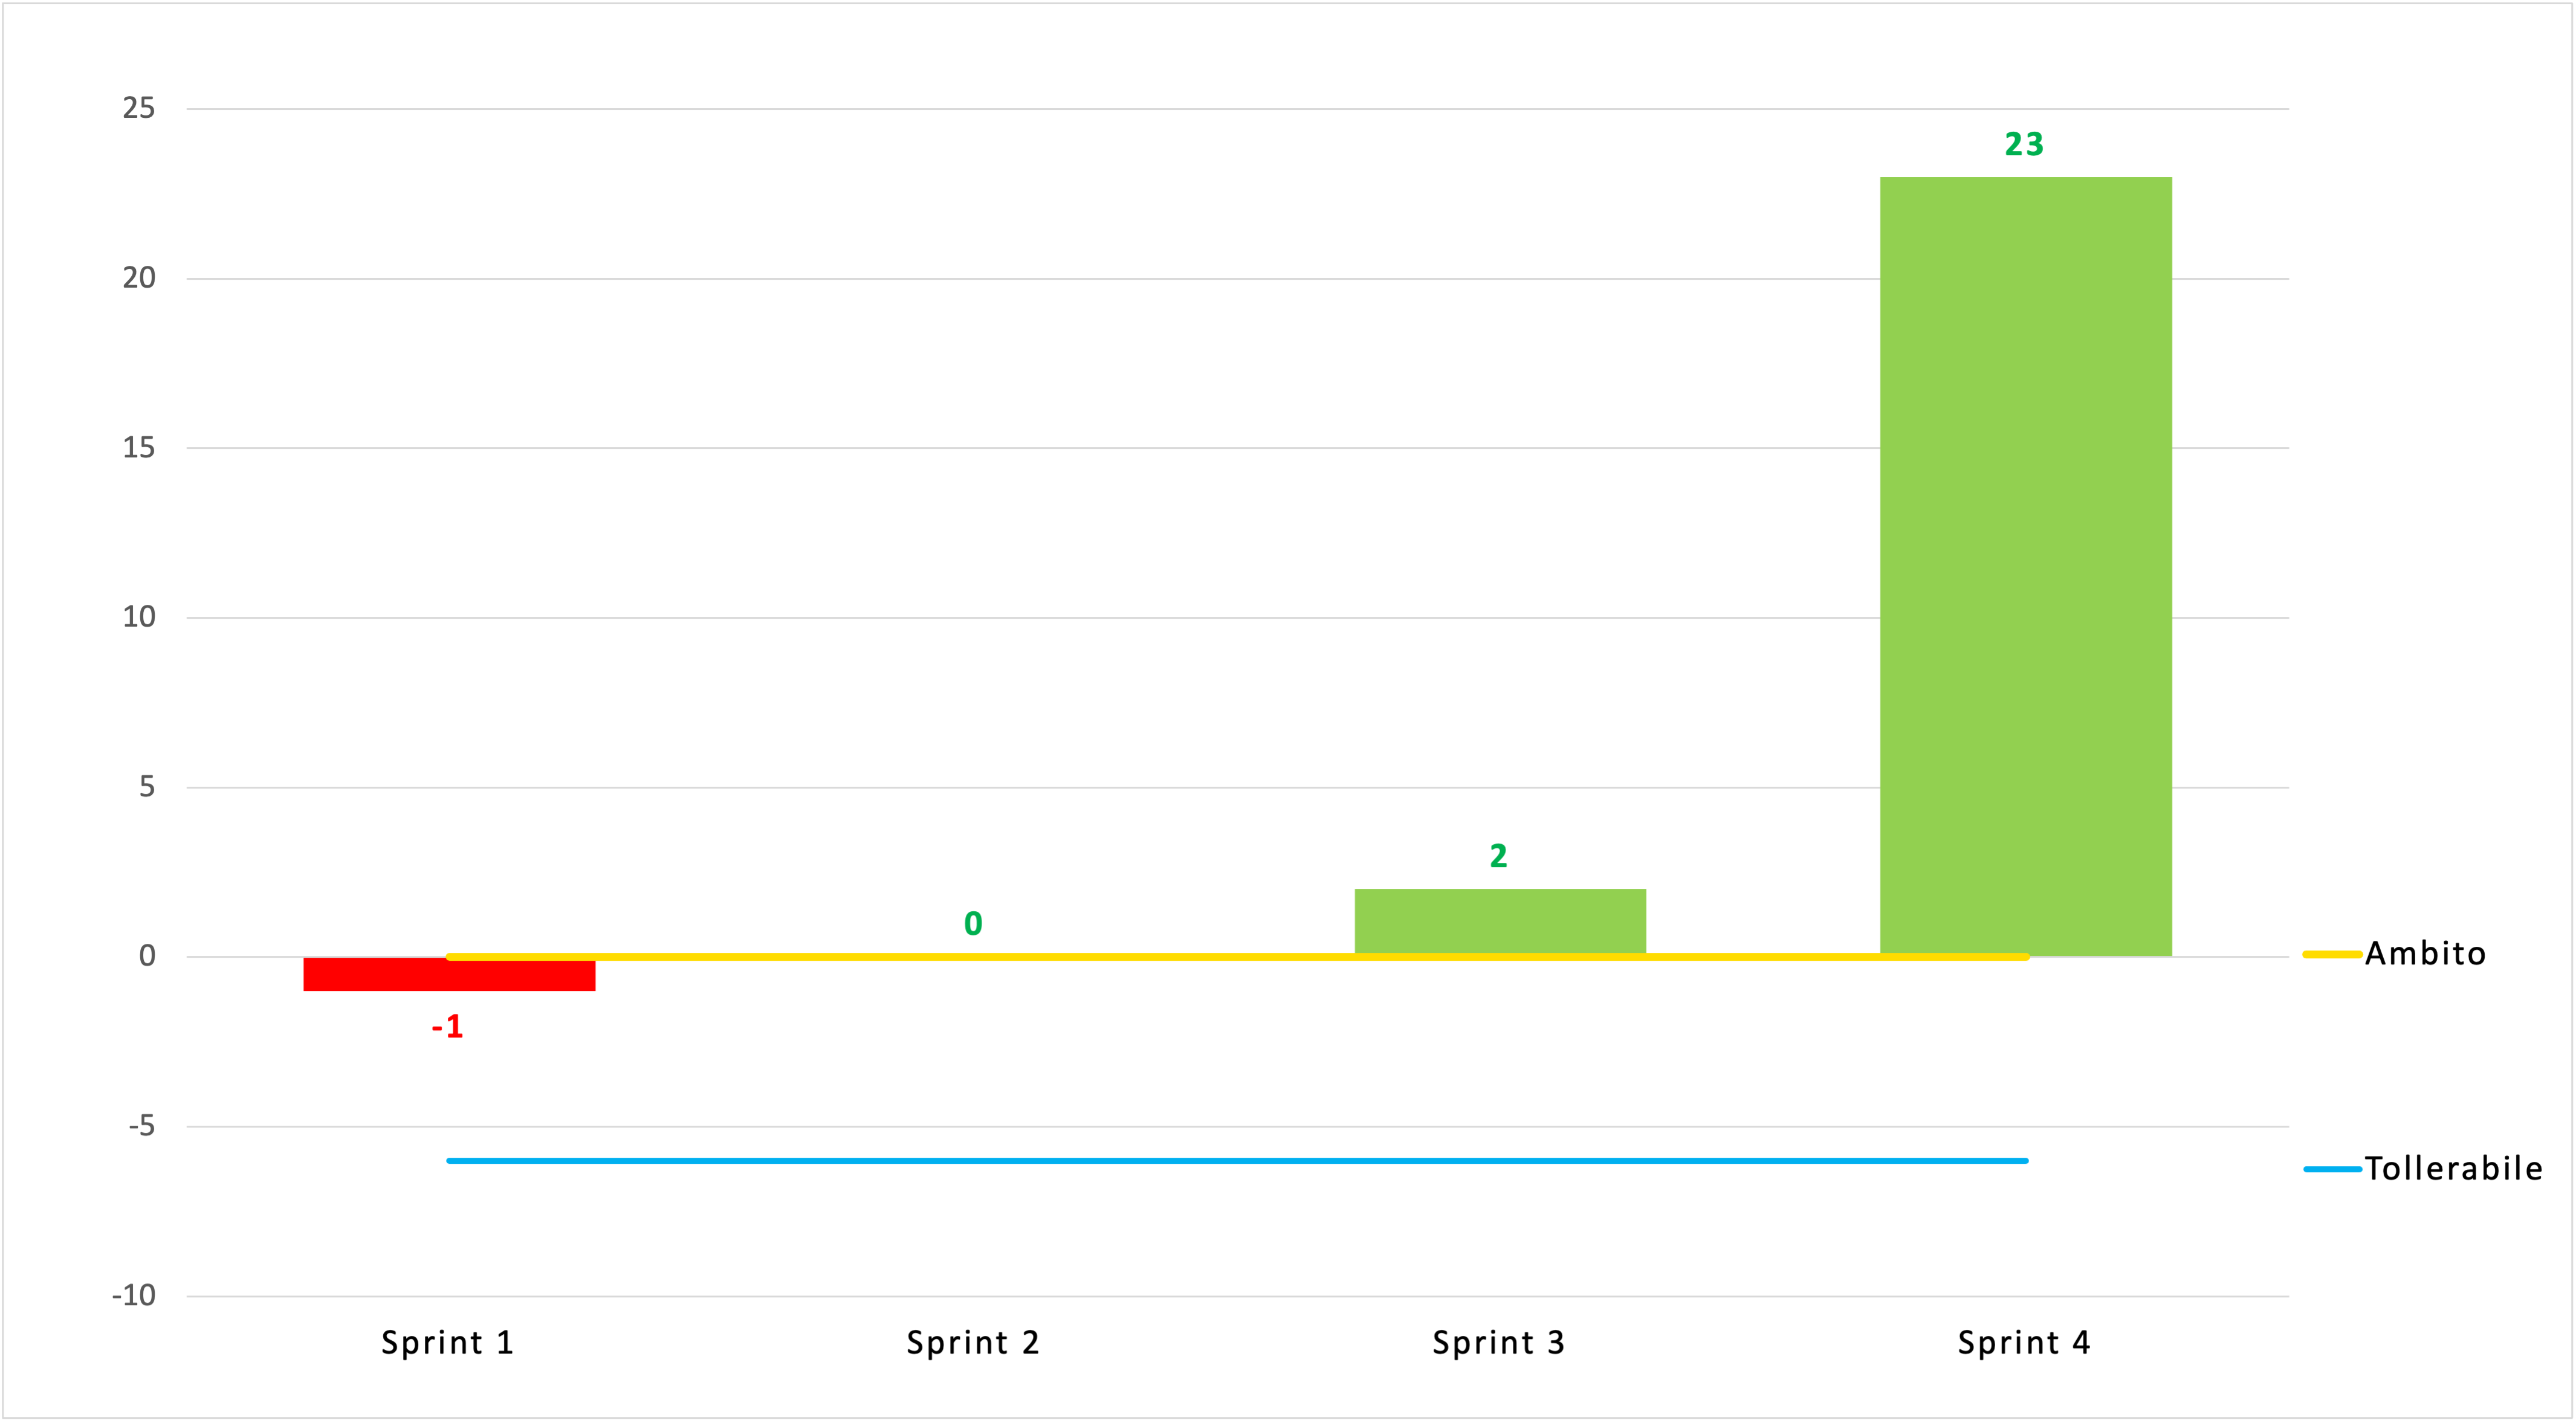
\includegraphics[width=15.5cm]{img/metriche/m3vp.png}
        \caption{M3VP - Variazione di piano. }
    \end{figure}
\subsection{M4VC}
\subsubsection{variazione di costo}
\begin{figure}[H]
        \centering        
        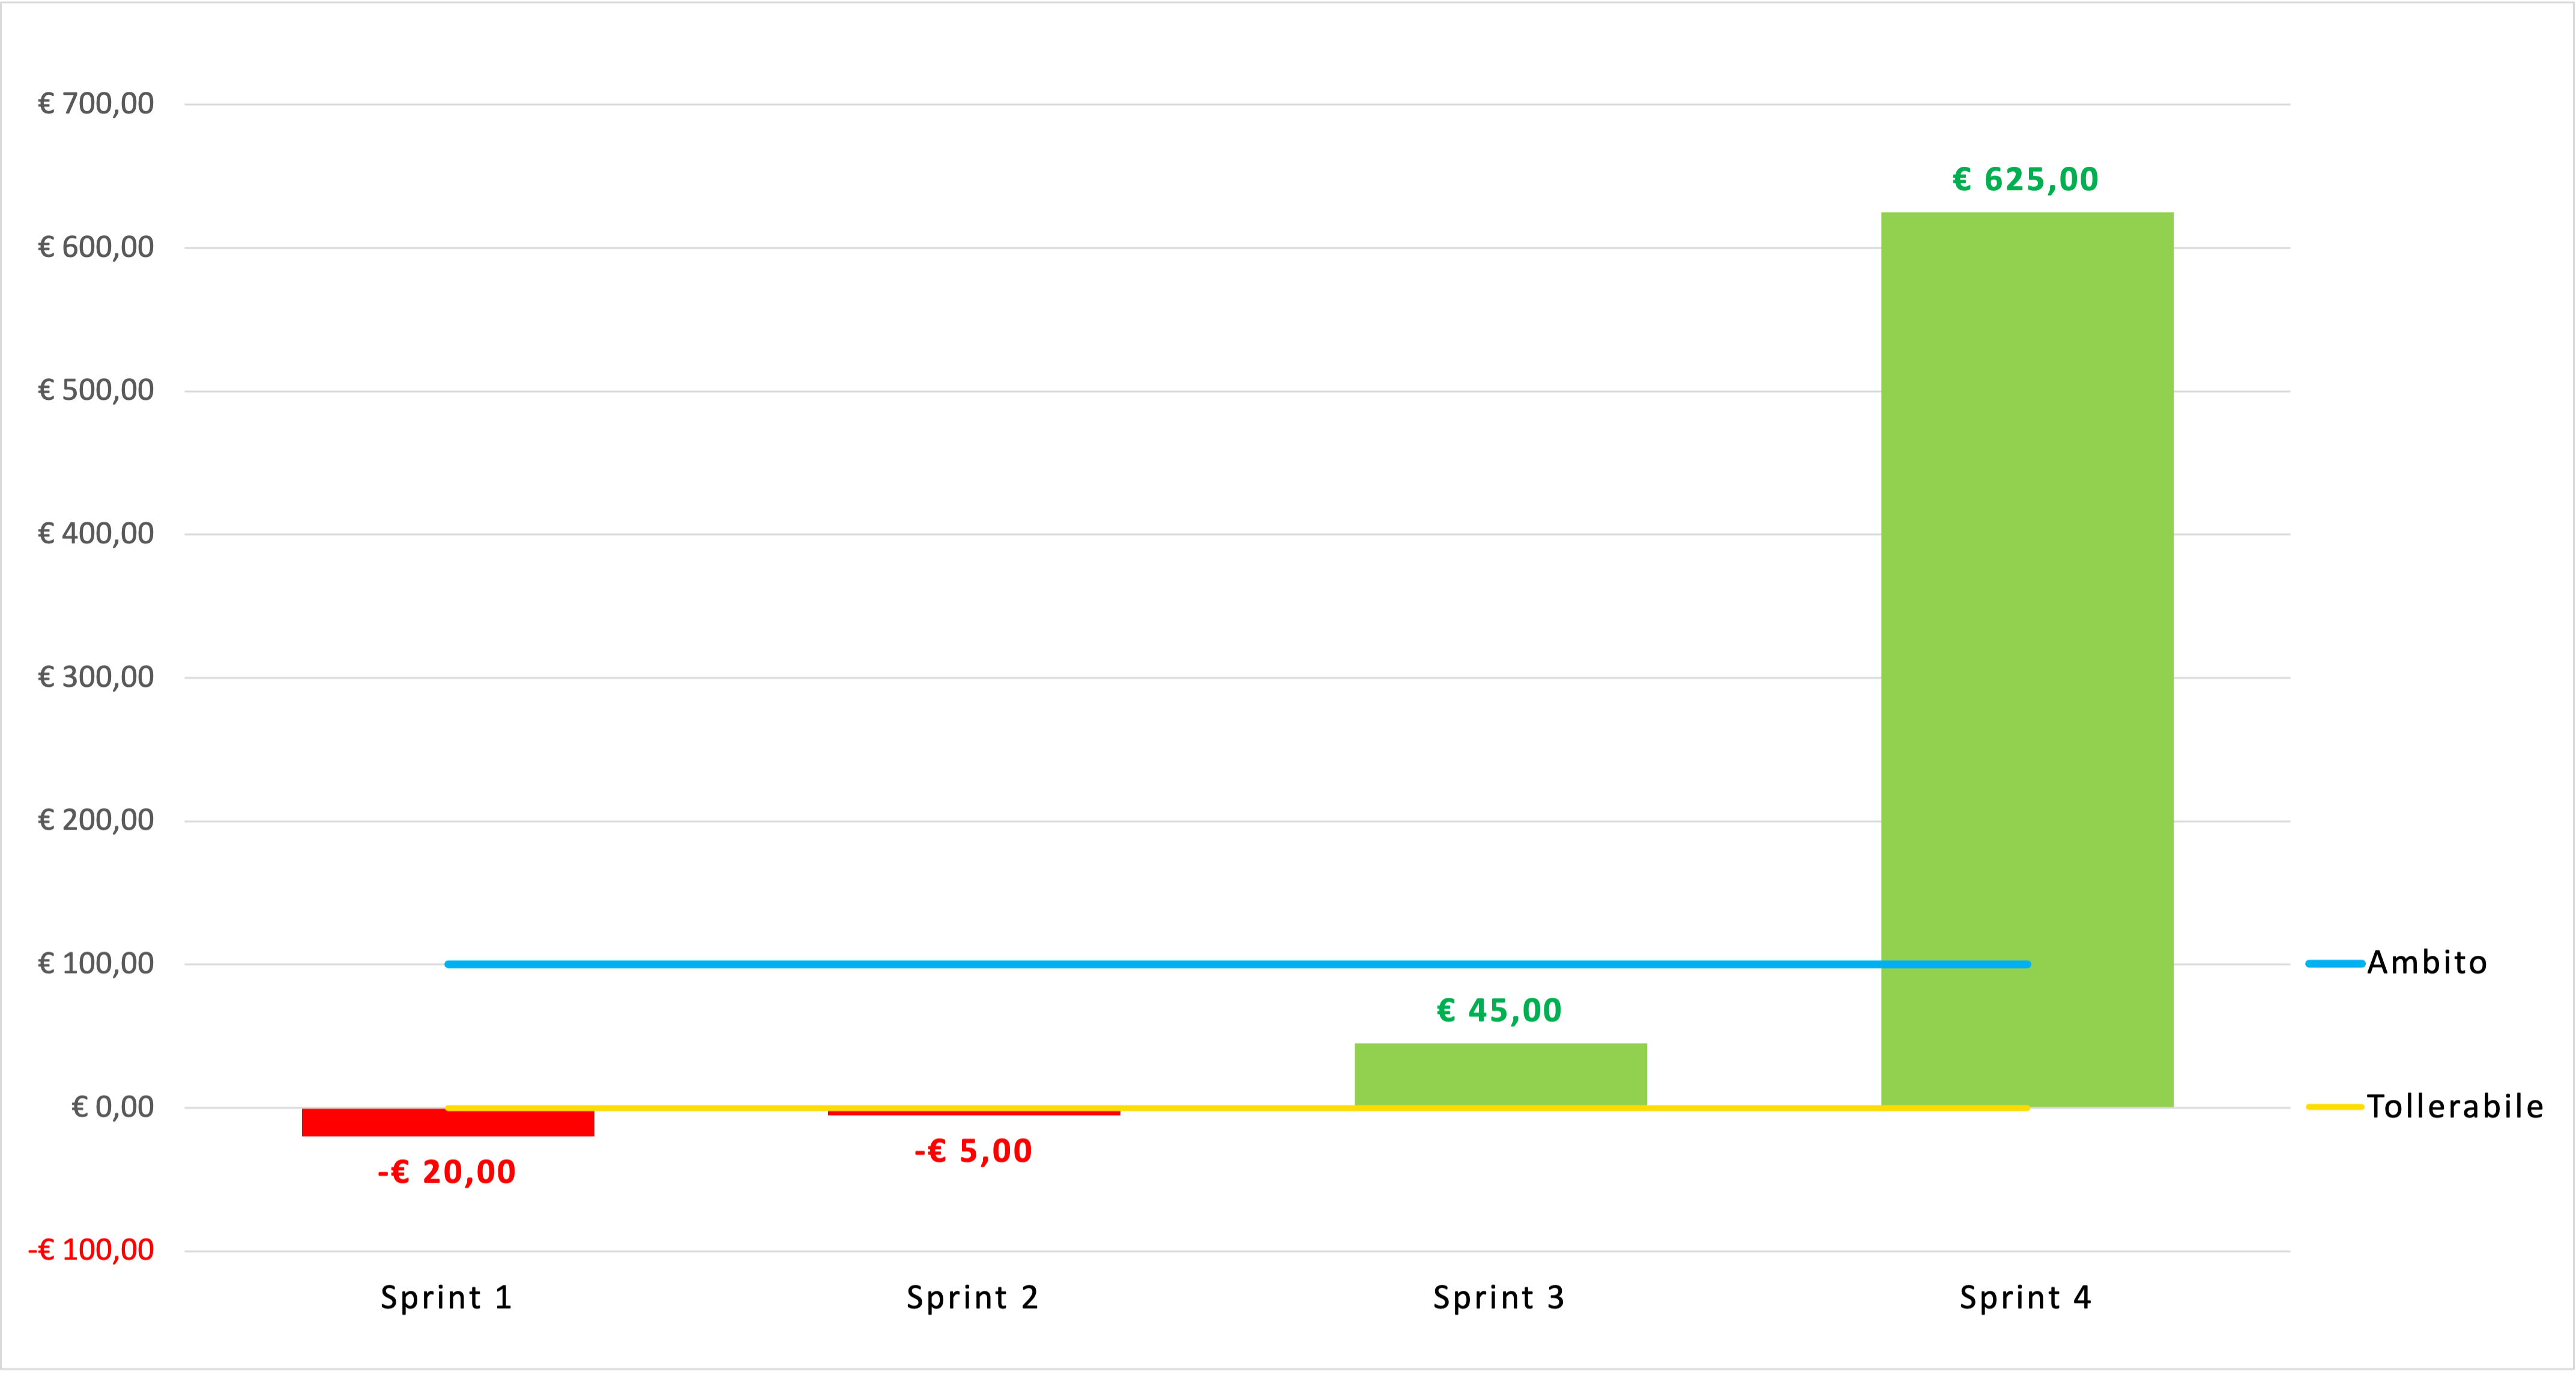
\includegraphics[width=15.5cm]{img/metriche/m4vc.png}
        \caption{M4VC - Variazione di costi. }
    \end{figure}
\subsection{M5ISR}
\subsection{M6CCM}
\subsection{M7SC}
\subsection{M8BC}
\subsection{M9IG}
\subsubsection{Analisi dei requisiti}
\subsubsection{Norme di progetto}
\subsubsection{Piano di progetto}

\subsubsection{Piano di qualifica}
\subsection{M10PRI}
\subsection{M11LMC}
\subsection{M12DC}

\subsection{Processi primari}

\subsection{Processi di supporto}
\begin{comment}
    \renewcommand{\arraystretch}{1.5}
    \begin{tabularx}{\textwidth}{p{0.05\textwidth}|p{0.35\textwidth}|X|X}
    \textbf{ID} & \textbf{Nome metrica} & \textbf{Valore accettabile} & \textbf{Valore ottimale}  \\
    \hline
    \multicolumn{4}{l}{\cellcolor{primarycolor}\textbf{\textit{Verifica}}} \\
    \hline
     &  &  &  \\
    \hline
     &  &  &  \\
    \hline
     &  &  &  \\
    \hline
     &  &  &  \\
    \hline
    \multicolumn{4}{l}{\cellcolor{primarycolor}\textbf{\textit{Gestione della qualità}}} \\
    \hline
     &  &  &  \\
    \end{tabularx}
  
\subsubsection{Documentazione}
    \renewcommand{\arraystretch}{1.5}
    \begin{tabularx}{\textwidth}{p{0.15\textwidth}|p{0.35\textwidth}|X|X}
    \textbf{ID} & \textbf{Nome metrica} & \textbf{Valore accettabile} & \textbf{Valore ottimale}  \\
    \hline
    \multicolumn{4}{l}{\cellcolor{primarycolor}\textbf{\textit{Funzionalità}}} \\
    \hline
    MPD-CR & Copertura dei requisiti & 100 & 100 \\
    
    \hline
   
    \multicolumn{4}{l}{\cellcolor{primarycolor}\textbf{\textit{Usabilità}}}
    \\
    \hline
     MPD-DIU & Difficoltà incontrate dall'utente & 2  & 0 \\
      
    \hline
   
    \multicolumn{4}{l}{\cellcolor{primarycolor}\textbf{\textit{Efficienza}}}
    \\
    \hline
     MPD-TA & Tempo di apprendimento & 10 minuti & 5 minuti \\
      \hline
     \multicolumn{4}{l}{\cellcolor{primarycolor}\textbf{\textit{Affidabiltà}}} \\
     MPD-TM & Tempo di risposta medio & 3 secondi & 2 secondi \\
      \hline
     \multicolumn{4}{l}{\cellcolor{primarycolor}\textbf{\textit{Portabiltà}}} \\
     MPD-VS & La capacità del programma di eseguire su più piattaforme & 100  & 100 \\
    \hline
     \multicolumn{4}{l}{\cellcolor{primarycolor}\textbf{\textit{Manutenibilità}}} \\
     MPD-CC & la capacità del software di essere modificato, 
     includendo correzioni, miglioramenti o adattamenti. & 30  & 45 \\
    \end{tabularx}
\end{comment}

\subsection{Processi organizzativi}

\section{Valutazioni per il miglioramento}
\begin{comment}
\section{Resoconto delle attività di verifica}

\subsection{Verifica della documentazione}
\subsubsection{Errori ortografici}
\subsubsection{Indici di Gulpease}

\subsection{Verifica dei processi}

\subsubsection{Estimated at completion}
\subsubsection{Budget variance e schedule variance}
\subsubsection{Actual cost e estimate to complete}
\subsubsection{Earned value e planned value}
\subsubsection{Requirements stability index e satisfied obligatory requirements}
\subsubsection{Code coverage back-end}
\subsubsection{Code coverage front-end}
\subsubsection{Passed test cases percentage}
\subsubsection{Failed test cases percentage}
\subsubsection{Comprensibilità del codice}
\end{comment}
\end{document}
